% Options for packages loaded elsewhere
\PassOptionsToPackage{unicode}{hyperref}
\PassOptionsToPackage{hyphens}{url}
%
\documentclass[
]{article}
\usepackage{amsmath,amssymb}
\usepackage{iftex}
\ifPDFTeX
  \usepackage[T1]{fontenc}
  \usepackage[utf8]{inputenc}
  \usepackage{textcomp} % provide euro and other symbols
\else % if luatex or xetex
  \usepackage{unicode-math} % this also loads fontspec
  \defaultfontfeatures{Scale=MatchLowercase}
  \defaultfontfeatures[\rmfamily]{Ligatures=TeX,Scale=1}
\fi
\usepackage{lmodern}
\ifPDFTeX\else
  % xetex/luatex font selection
\fi
% Use upquote if available, for straight quotes in verbatim environments
\IfFileExists{upquote.sty}{\usepackage{upquote}}{}
\IfFileExists{microtype.sty}{% use microtype if available
  \usepackage[]{microtype}
  \UseMicrotypeSet[protrusion]{basicmath} % disable protrusion for tt fonts
}{}
\makeatletter
\@ifundefined{KOMAClassName}{% if non-KOMA class
  \IfFileExists{parskip.sty}{%
    \usepackage{parskip}
  }{% else
    \setlength{\parindent}{0pt}
    \setlength{\parskip}{6pt plus 2pt minus 1pt}}
}{% if KOMA class
  \KOMAoptions{parskip=half}}
\makeatother
\usepackage{xcolor}
\usepackage[margin=1in]{geometry}
\usepackage{longtable,booktabs,array}
\usepackage{calc} % for calculating minipage widths
% Correct order of tables after \paragraph or \subparagraph
\usepackage{etoolbox}
\makeatletter
\patchcmd\longtable{\par}{\if@noskipsec\mbox{}\fi\par}{}{}
\makeatother
% Allow footnotes in longtable head/foot
\IfFileExists{footnotehyper.sty}{\usepackage{footnotehyper}}{\usepackage{footnote}}
\makesavenoteenv{longtable}
\usepackage{graphicx}
\makeatletter
\newsavebox\pandoc@box
\newcommand*\pandocbounded[1]{% scales image to fit in text height/width
  \sbox\pandoc@box{#1}%
  \Gscale@div\@tempa{\textheight}{\dimexpr\ht\pandoc@box+\dp\pandoc@box\relax}%
  \Gscale@div\@tempb{\linewidth}{\wd\pandoc@box}%
  \ifdim\@tempb\p@<\@tempa\p@\let\@tempa\@tempb\fi% select the smaller of both
  \ifdim\@tempa\p@<\p@\scalebox{\@tempa}{\usebox\pandoc@box}%
  \else\usebox{\pandoc@box}%
  \fi%
}
% Set default figure placement to htbp
\def\fps@figure{htbp}
\makeatother
\setlength{\emergencystretch}{3em} % prevent overfull lines
\providecommand{\tightlist}{%
  \setlength{\itemsep}{0pt}\setlength{\parskip}{0pt}}
\setcounter{secnumdepth}{-\maxdimen} % remove section numbering
\usepackage{bookmark}
\IfFileExists{xurl.sty}{\usepackage{xurl}}{} % add URL line breaks if available
\urlstyle{same}
\hypersetup{
  pdftitle={Supplementary Information},
  hidelinks,
  pdfcreator={LaTeX via pandoc}}

\title{\textbf{Supplementary Information}}
\usepackage{etoolbox}
\makeatletter
\providecommand{\subtitle}[1]{% add subtitle to \maketitle
  \apptocmd{\@title}{\par {\large #1 \par}}{}{}
}
\makeatother
\subtitle{BIOREDIS: rapid and customizable design of nucleic acid
therapeutics}
\author{}
\date{\vspace{-2.5em}}

\begin{document}
\maketitle

\hfill\break

\section{Supplementary Tables}\label{supplementary-tables}

\subsection{Codons optimisation}\label{codons-optimisation}

\begin{longtable}[]{@{}
  >{\raggedright\arraybackslash}p{(\linewidth - 12\tabcolsep) * \real{0.2048}}
  >{\raggedright\arraybackslash}p{(\linewidth - 12\tabcolsep) * \real{0.0602}}
  >{\raggedleft\arraybackslash}p{(\linewidth - 12\tabcolsep) * \real{0.0964}}
  >{\raggedleft\arraybackslash}p{(\linewidth - 12\tabcolsep) * \real{0.0602}}
  >{\raggedleft\arraybackslash}p{(\linewidth - 12\tabcolsep) * \real{0.1928}}
  >{\raggedleft\arraybackslash}p{(\linewidth - 12\tabcolsep) * \real{0.2048}}
  >{\raggedleft\arraybackslash}p{(\linewidth - 12\tabcolsep) * \real{0.1807}}@{}}
\toprule\noalign{}
\begin{minipage}[b]{\linewidth}\raggedright
tool
\end{minipage} & \begin{minipage}[b]{\linewidth}\raggedright
gene
\end{minipage} & \begin{minipage}[b]{\linewidth}\raggedleft
GC
\end{minipage} & \begin{minipage}[b]{\linewidth}\raggedleft
freq
\end{minipage} & \begin{minipage}[b]{\linewidth}\raggedleft
changed\_bases \%
\end{minipage} & \begin{minipage}[b]{\linewidth}\raggedleft
changed\_codons \%
\end{minipage} & \begin{minipage}[b]{\linewidth}\raggedleft
MFE {[}kcal/mol{]}
\end{minipage} \\
\midrule\noalign{}
\endhead
\bottomrule\noalign{}
\endlastfoot
Native & KIT & 44.9588 & 0.38 & 0 & 0.0 & -777.3 \\
Native & PAX3 & 57.6733 & 0.38 & 0 & 0.0 & -383.3 \\
BIOREDIS & KIT & 59.2936 & 0.46 & 24 & 62.0 & -1015.3 \\
BIOREDIS & PAX3 & 57.9208 & 0.41 & 23 & 56.9 & -403.8 \\
CodonTransformer & KIT & 55.4184 & 0.44 & 21 & 56.0 & -1006.1 \\
CodonTransformer & PAX3 & 61.4686 & 0.41 & 20 & 51.0 & -452.2 \\
GenScript & KIT & 54.8354 & 0.44 & 23 & 60.0 & -893.3 \\
GenScript & PAX3 & 58.2508 & 0.41 & 22 & 54.0 & -362.4 \\
VectorBuilder & KIT & 54.8011 & 0.44 & 23 & 59.0 & -922.8 \\
VectorBuilder & PAX3 & 58.9109 & 0.41 & 22 & 55.0 & -396.7 \\
\end{longtable}

\textbf{Table S1:} Data including statistics of the native sequences
(\emph{KIT, PAX3}) and optimized sequences generated using various
tools.

\hfill\break

\begin{longtable}[]{@{}llrrr@{}}
\toprule\noalign{}
source & RNAi\_seq & specificity & GC\% & score \\
\midrule\noalign{}
\endhead
\bottomrule\noalign{}
\endlastfoot
BIOREDIS & ATAACAGCCTAATCTCGTCGC & 1 & 47.62 & 10 \\
BIOREDIS & TAACAGCCTAATCTCGTCGCC & 1 & 52.38 & 8 \\
BIOREDIS & TATTCTCATTCGTTTCATCCA & 1 & 33.33 & 7 \\
BIOREDIS & TGTAGAACTTAGAATCGACCG & 1 & 42.86 & 7 \\
BIOREDIS & TCATAAGGAAGTTGTGTTGGG & 1 & 42.86 & 7 \\
BIOREDIS & ATATTGGGCAGTGAGGAAGGG & 1 & 52.38 & 7 \\
BIOREDIS & ATATACAAGTGCTGGCTAGGG & 1 & 47.62 & 7 \\
BIOREDIS & GAAAGACAGGATTGCAGTGGG & 1 & 52.38 & 7 \\
BIOREDIS & TTTGTAGGTCAGAATCATCAC & 1 & 38.10 & 6 \\
BIOREDIS & CATTCTGCTTATTCTCATTCG & 1 & 38.10 & 6 \\
Eurofins Genomics & TTCTGCTTATTCTCATTCG & 1 & 36.84 & 6 \\
Eurofins Genomics & TATATGGCTCTTAATCTAC & 1 & 31.58 & 1 \\
Eurofins Genomics & TCTATAACTAACAACCACT & 1 & 31.58 & 1 \\
Eurofins Genomics & TTATCTACTACTTCCAAGG & 1 & 36.84 & 6 \\
Eurofins Genomics & TTAATTAAGCCATAAGCAG & 1 & 31.58 & 4 \\
Eurofins Genomics & TTCTGCATGATCTTCCTGC & 1 & 47.37 & 4 \\
Eurofins Genomics & TCTTGTATCATCATACTAC & 1 & 31.58 & -1 \\
Eurofins Genomics & TGTATGAACACGGACAATT & 1 & 36.84 & -2 \\
Eurofins Genomics & TATAGATCCACTGCTGGTG & 1 & 47.37 & 4 \\
Eurofins Genomics & TTAATCTCGTTAGATGAAG & 1 & 31.58 & 1 \\
GenScript & ACTATCGCAGGAAGACTCCTT & 0 & 47.62 & 0 \\
GenScript & TGGTAGGCGCGTTTCACACTT & 1 & 52.38 & -2 \\
GenScript & TGTATACAGAAACGAAACCTT & 1 & 33.33 & 1 \\
GenScript & AGAACTCTGAACCACTAGCTT & 1 & 42.86 & 1 \\
GenScript & GTCTAAATAACAGAGTGCCTT & 1 & 38.10 & -2 \\
GenScript & GAAACGAAACCTTATGGTGTT & 1 & 38.10 & 2 \\
GenScript & AGTCATGGCCGCATCTGACTT & 1 & 52.38 & 0 \\
GenScript & TTCCAAGGTTGTTGTGACATT & 1 & 38.10 & -1 \\
GenScript & CTCGTTAGATGAAGTTCACTT & 1 & 38.10 & -1 \\
GenScript & GCACGTGTATTTGCCGGTGTT & 1 & 52.38 & -1 \\
Invivogen & AGTACTATCGCAGGAAGACTC & 0 & 47.62 & 2 \\
Invivogen & ATAACAGCCTAATCTCGTCGC & 1 & 47.62 & 10 \\
Invivogen & TAACAGCCTAATCTCGTCGCC & 1 & 52.38 & 8 \\
Invivogen & TTATTCTCATTCGTTTCATCC & 1 & 33.33 & 6 \\
Invivogen & TTGTAGAACTTAGAATCGACC & 1 & 38.10 & 3 \\
Invivogen & TTTACAGCGACAGTCATGGCC & 1 & 52.38 & 7 \\
Invivogen & ATCTCTTTCTATGTATGAGCC & 1 & 38.10 & 6 \\
Invivogen & TATTTGTAGGTCAGAATCATC & 1 & 33.33 & 2 \\
Invivogen & TTTGAGTTCAGACATGAGGGC & 1 & 47.62 & 8 \\
Invivogen & ATAACAGAGTGCCTTAAGTGC & 1 & 42.86 & 6 \\
Invivogen & ATTCTTGGAGGCGAGGAAAGC & 1 & 52.38 & 5 \\
Invivogen & ATAGATCCACTGCTGGTGTTC & 1 & 47.62 & 2 \\
Invivogen & TGGTAAGCTACTCTAGACAGC & 1 & 47.62 & 1 \\
VectorBuilder & ATAATTGGTCACTTCTGGGTC & 1 & 42.86 & 5 \\
VectorBuilder & ATATTTCTCCTGTAGTTTAGT & 1 & 28.57 & 4 \\
VectorBuilder & AATAAACCTCAAGTCCTTGGG & 1 & 42.86 & 9 \\
VectorBuilder & ATATTACTTTCATTCTCAGAC & 1 & 28.57 & 3 \\
VectorBuilder & TTTATTGTGCACGTCACTGTG & 1 & 42.86 & 6 \\
VectorBuilder & TTTAATCTCGTTAGATGAAGT & 1 & 28.57 & 3 \\
VectorBuilder & ATAATTGAAGTCACCGTGATG & 1 & 38.10 & 2 \\
VectorBuilder & ATTATTGGCATAACACATGAA & 1 & 28.57 & 2 \\
VectorBuilder & ATAAATGGAATTGCTTAAGCC & 1 & 33.33 & 8 \\
VectorBuilder & ATTTATCAGTGAAGGTTCTGT & 1 & 33.33 & 3 \\
\end{longtable}

\textbf{Table S2:} Data including statistics of the predicted RNAi of
\emph{KIT} gene using various tools.

\newpage

\begin{longtable}[]{@{}llrrr@{}}
\toprule\noalign{}
source & RNAi\_seq & specificity & GC\% & score \\
\midrule\noalign{}
\endhead
\bottomrule\noalign{}
\endlastfoot
BIOREDIS & AATTATATCCAGGTGAAGGCG & 1 & 42.86 & 8 \\
BIOREDIS & AAATTATATCCAGGTGAAGGC & 1 & 38.10 & 8 \\
BIOREDIS & TTTACTTCTCAGGATGCGGCT & 1 & 47.62 & 7 \\
BIOREDIS & ATTTACTTCTCAGGATGCGGC & 1 & 47.62 & 7 \\
BIOREDIS & AATTTACTTCTCAGGATGCGG & 1 & 42.86 & 7 \\
BIOREDIS & TTCAGAGTCAATATCAGAGCC & 1 & 42.86 & 6 \\
BIOREDIS & TTCTTCTCGCTTTCCTCTGCC & 1 & 52.38 & 6 \\
BIOREDIS & AAGTTTGGTACGAGTCTGGGC & 1 & 52.38 & 6 \\
BIOREDIS & TATCCAGGTGAAGGCGAAACG & 1 & 52.38 & 6 \\
BIOREDIS & TGAAGGCGAAACGGAAAGGCG & 1 & 57.14 & 6 \\
Eurofins Genomics & TTCTTCTCCACGTCAGGCG & 1 & 57.89 & 6 \\
Eurofins Genomics & TCTTCCTCTTCTCCACTGC & 1 & 52.63 & 3 \\
Eurofins Genomics & TGTTCTAGCTCCTCGATGA & 1 & 47.37 & 2 \\
Eurofins Genomics & TTCCTCTTCTCCACTGCTT & 1 & 47.37 & 0 \\
Eurofins Genomics & TACAACACATTGTTGTTGG & 1 & 36.84 & 6 \\
Eurofins Genomics & TATCAGAGCCTTCATCTGA & 1 & 42.11 & 3 \\
Eurofins Genomics & TGTTCTGCTGTGAAGGTGG & 1 & 52.63 & 3 \\
Eurofins Genomics & GTCAAGGATTCCTCCATTC & 1 & 47.37 & -1 \\
Eurofins Genomics & TATGTGAATGCATGTCACT & 1 & 36.84 & 4 \\
Eurofins Genomics & CATGTGAACACTTCTGTTC & 1 & 42.11 & 1 \\
GenScript & CAGAGTCAATATCAGAGCCTT & 1 & 42.86 & -1 \\
GenScript & ACCATGTGAAACCATTGCCTT & 1 & 42.86 & 0 \\
GenScript & TCGATCACAGACCGCGTCCTT & 1 & 57.14 & -1 \\
GenScript & GTGCTTTGGTGTACAGTGCTT & 1 & 47.62 & -2 \\
GenScript & GTCAGGCGTTGTCACCTGCTT & 1 & 57.14 & -2 \\
GenScript & AGGATTCCTCCATTCTTGCTT & 1 & 42.86 & -2 \\
GenScript & CCTTTACAGCTAGTCTAGCTT & 1 & 42.86 & -2 \\
GenScript & ACTCGCTACGTCATAGTTCTT & 1 & 42.86 & 1 \\
GenScript & ACTCACTGACGGCACGGTGTT & 1 & 57.14 & 1 \\
GenScript & GCTGTGAAGGTGGTTCGGCTT & 1 & 57.14 & -1 \\
Invivogen & AAGTTTGGTACGAGTCTGGGC & 1 & 52.38 & 6 \\
Invivogen & AACTAAATTCGGTACTATGTC & 1 & 33.33 & 3 \\
Invivogen & ATTTGTCTCGGATTTCCCAGC & 1 & 47.62 & 6 \\
Invivogen & TTCACTTACGCGATATCTGGC & 1 & 47.62 & 6 \\
Invivogen & TTATATCGCCTTGGGCATTGC & 1 & 47.62 & 6 \\
VectorBuilder & AATTTACTTCTCAGGATGCGG & 1 & 42.86 & 7 \\
VectorBuilder & AAATAACACTGCCTTCCACCT & 1 & 42.86 & 6 \\
VectorBuilder & TTATATCCAGGTGAAGGCGAA & 1 & 42.86 & 1 \\
VectorBuilder & TTTATTGCTCCAGGTCTTCCT & 1 & 42.86 & 7 \\
VectorBuilder & TATTTAGGAGGTCCTTTACAG & 1 & 38.10 & 4 \\
VectorBuilder & ATAAATGTCAGGGTAATGAGT & 1 & 33.33 & 3 \\
VectorBuilder & TTATTTCAATTTCCAGTGTGT & 1 & 28.57 & 3 \\
VectorBuilder & AATTATCTGATCTGGTCTCTA & 1 & 33.33 & 3 \\
VectorBuilder & TAATTTGTCTCGGATTTCCCA & 1 & 38.10 & 6 \\
VectorBuilder & TTATATCGCCTTGGGCATTGC & 1 & 47.62 & 6 \\
\end{longtable}

\textbf{Table S3:} Data including statistics of the predicted RNAi of
\emph{PAX3} gene using various tools.

\newpage

\section{Supplementary Figures}\label{supplementary-figures}

\begin{center}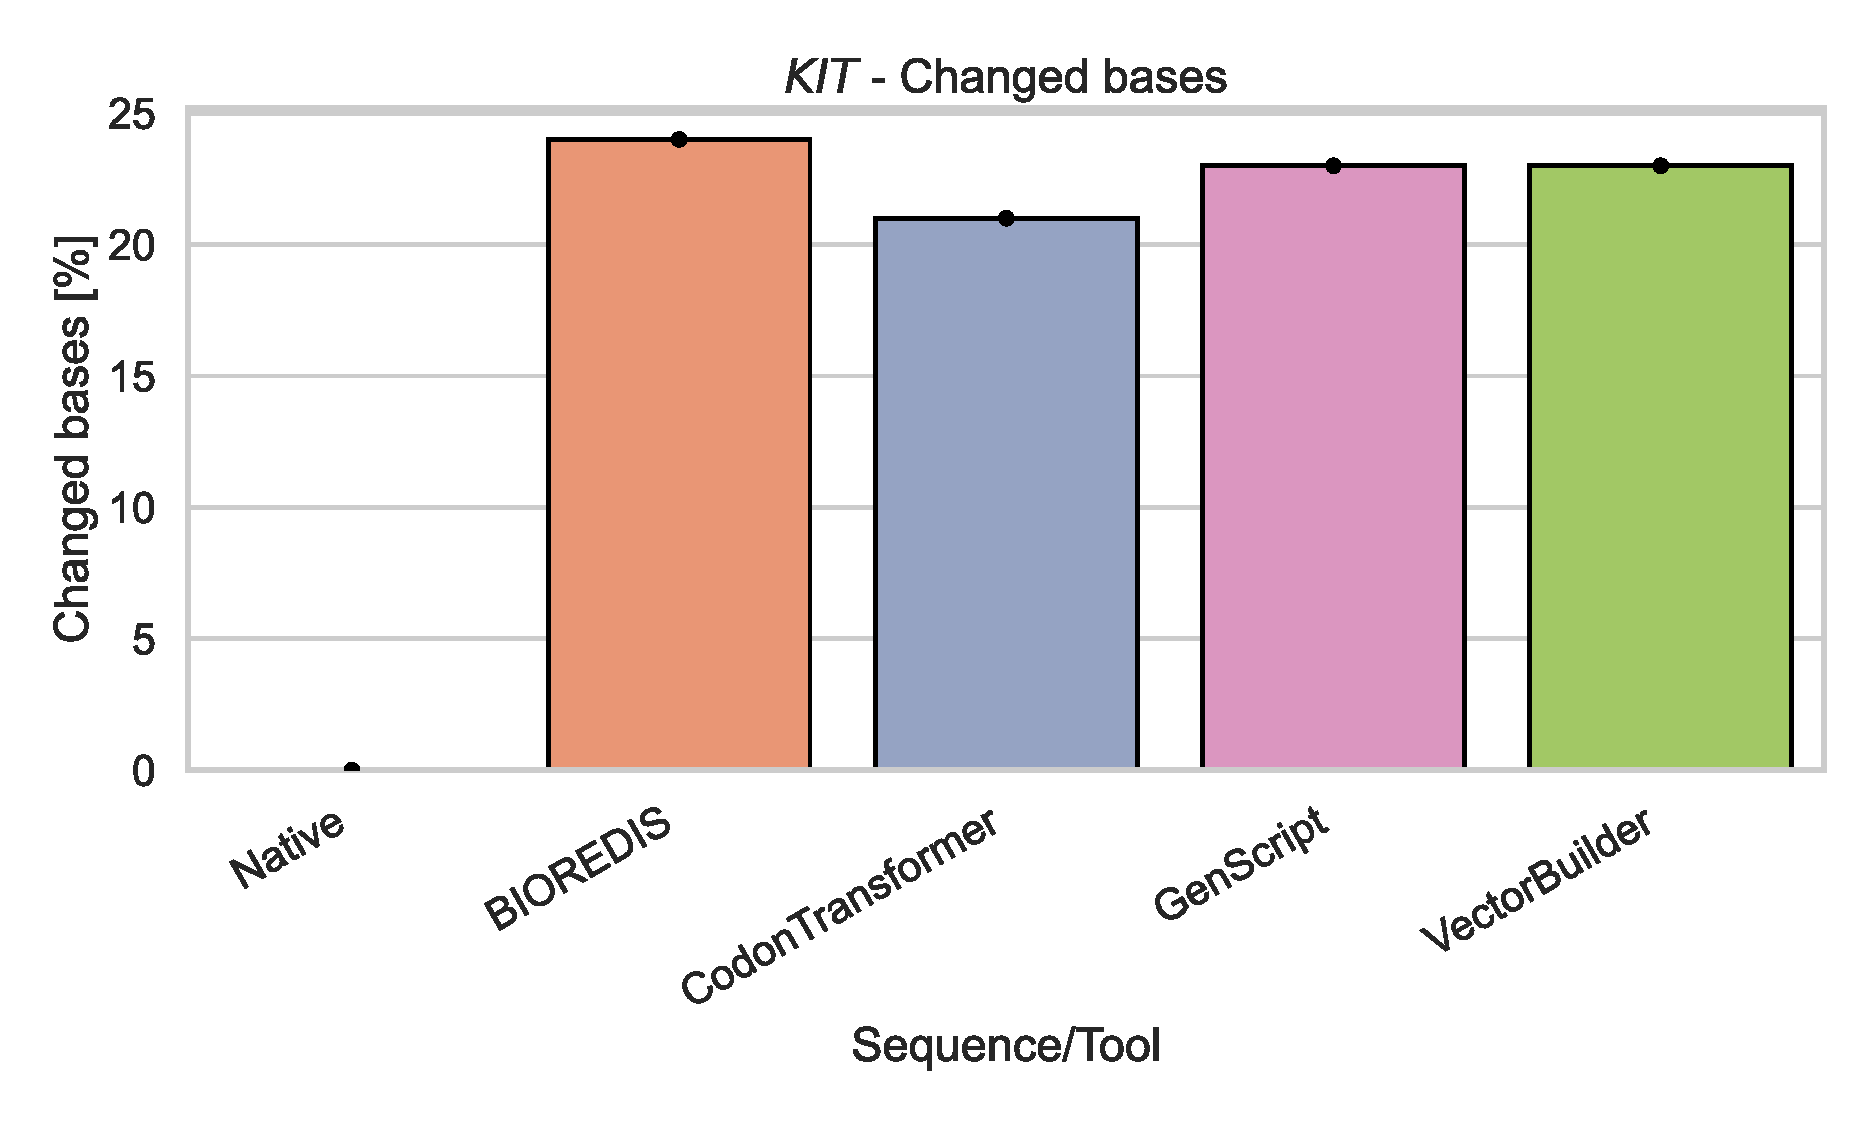
\includegraphics[width=0.8\linewidth]{supplemetary_figures/Supp.Fig.1-KIT} \end{center}

\begin{center}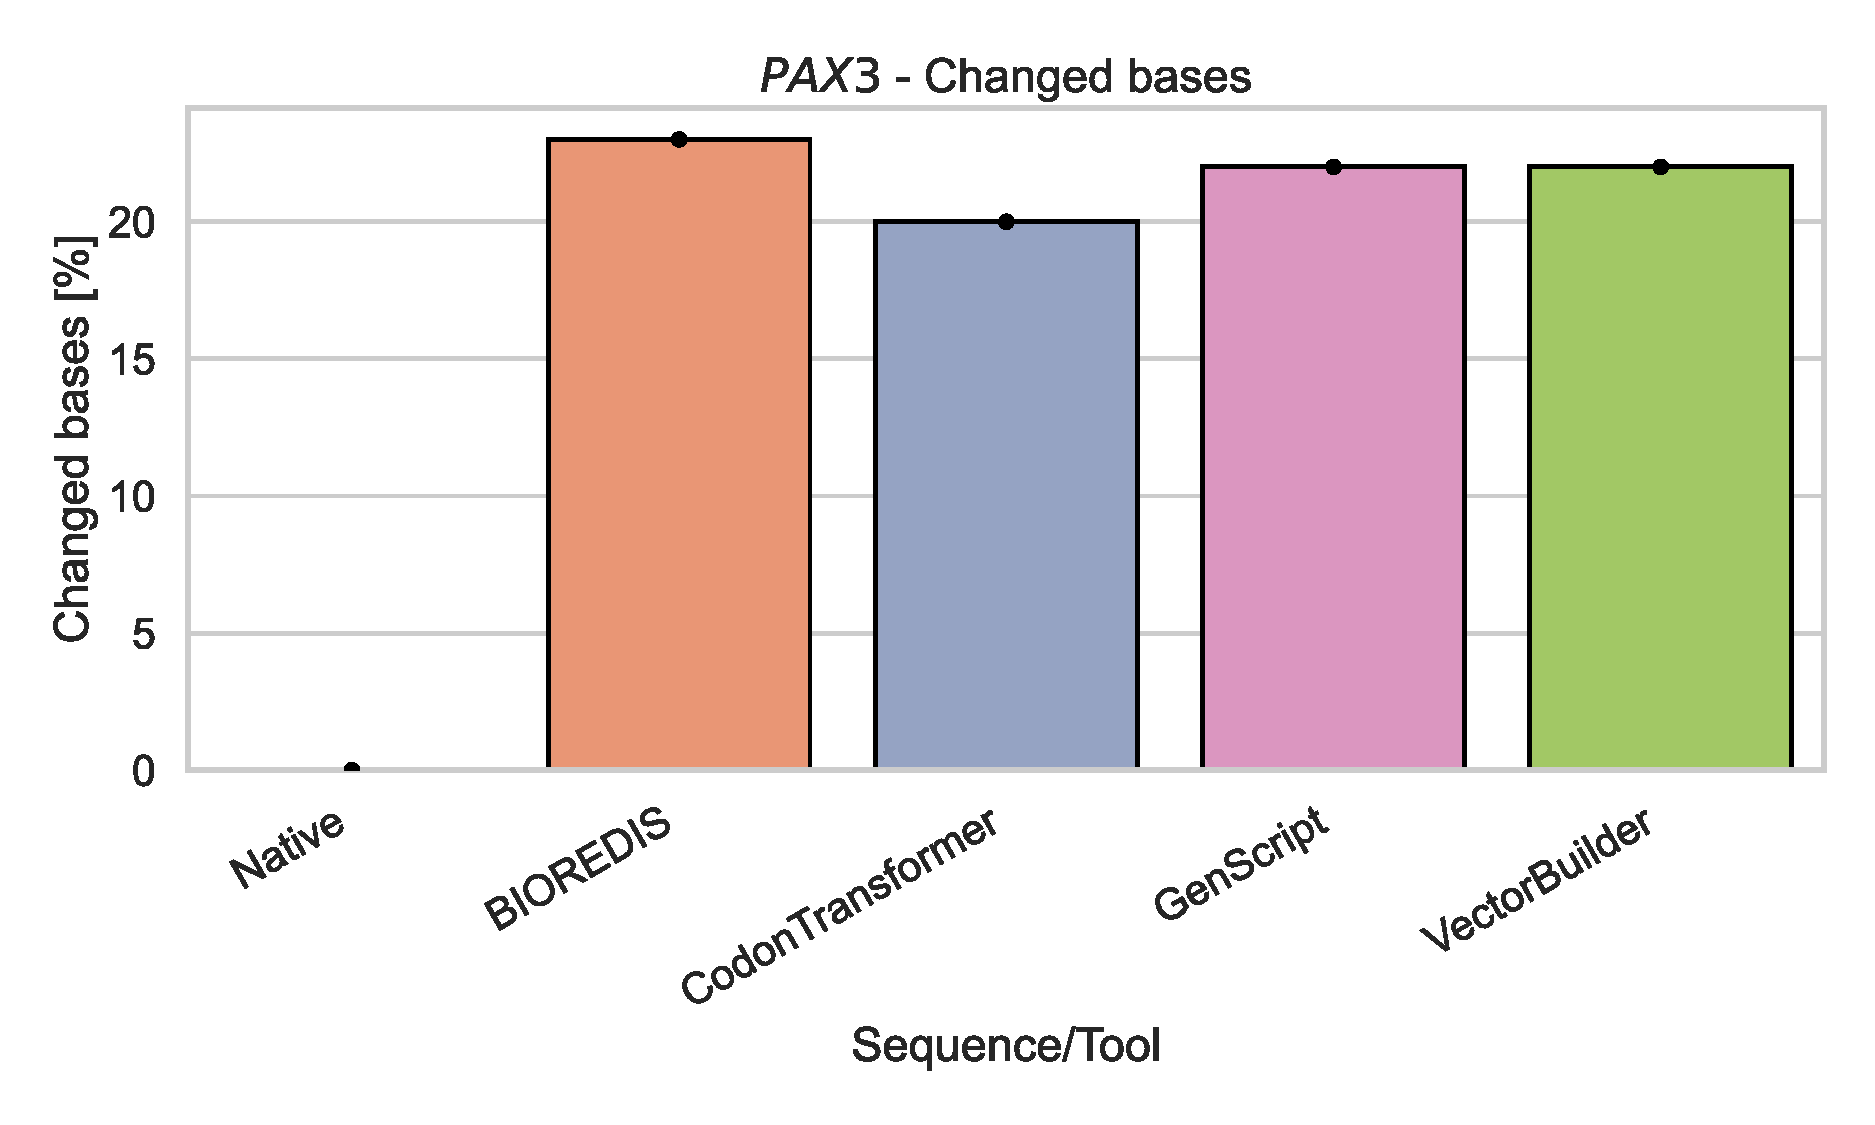
\includegraphics[width=0.8\linewidth]{supplemetary_figures/Supp.Fig.1-PAX3} \end{center}

\textbf{Figure S1.} Percent of nucleotide changes in optimised sequences
relative to the native sequence of the \emph{KIT} and \emph{PAX3} genes.

\newpage

\begin{center}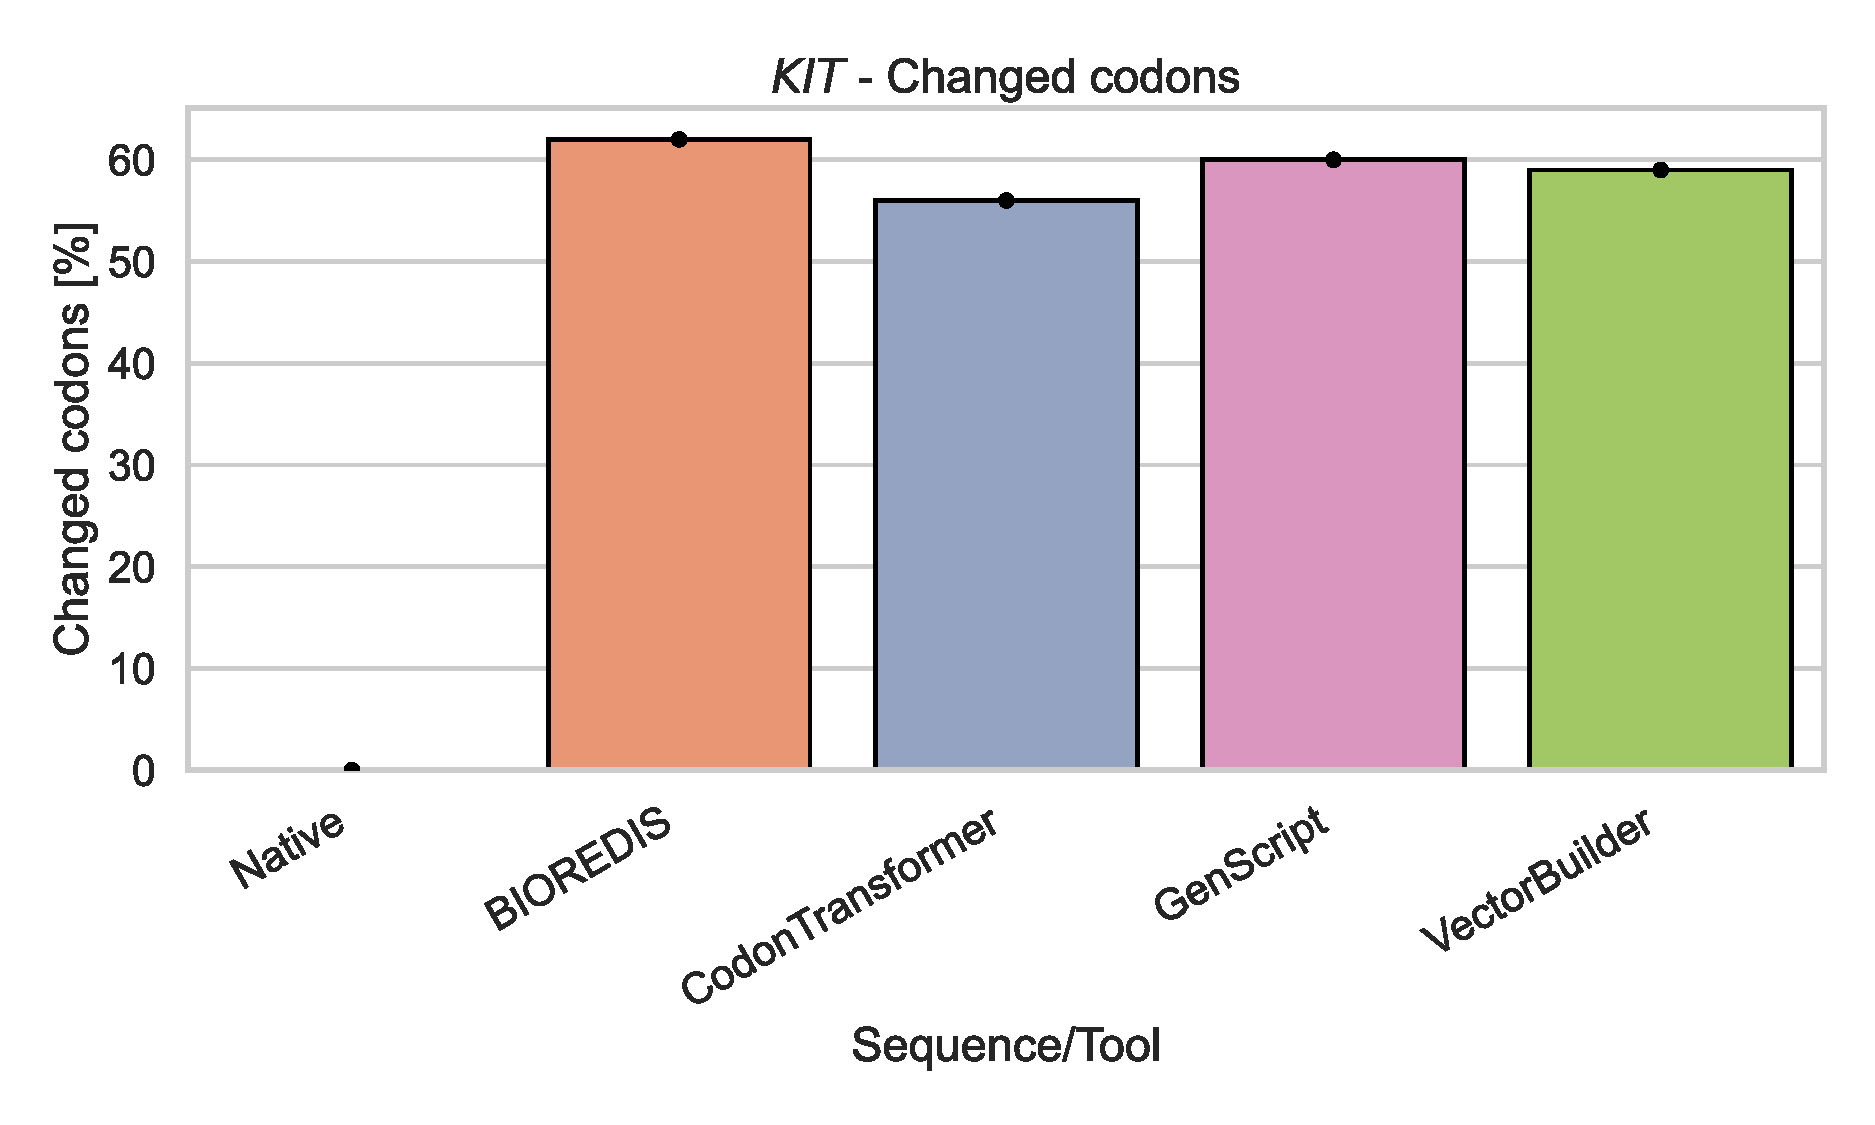
\includegraphics[width=0.8\linewidth]{supplemetary_figures/Supp.Fig.2-KIT} \end{center}

\begin{center}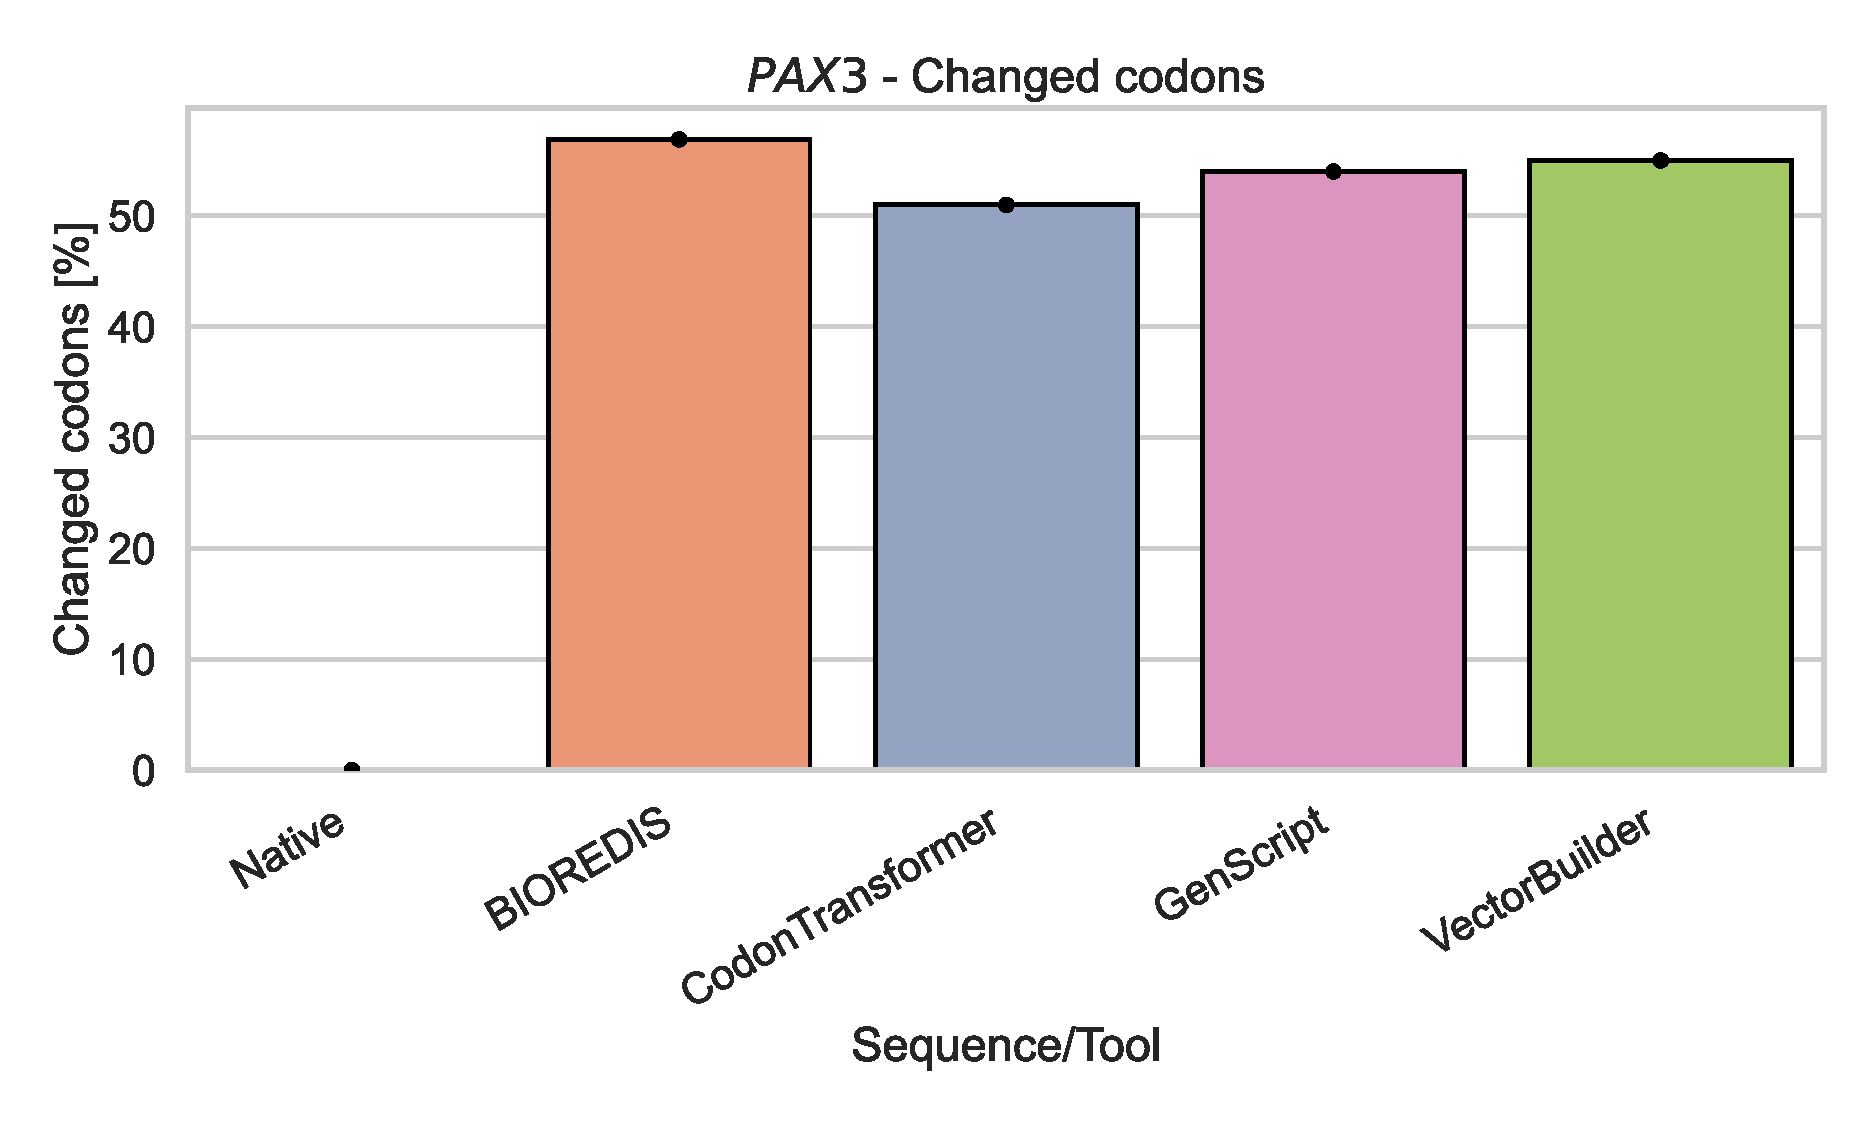
\includegraphics[width=0.8\linewidth]{supplemetary_figures/Supp.Fig.2-PAX3} \end{center}

\textbf{Figure S2.} Percent of codon changes in optimised sequences
relative to the native sequence of the \emph{KIT} and \emph{PAX3} genes.

\newpage

\begin{center}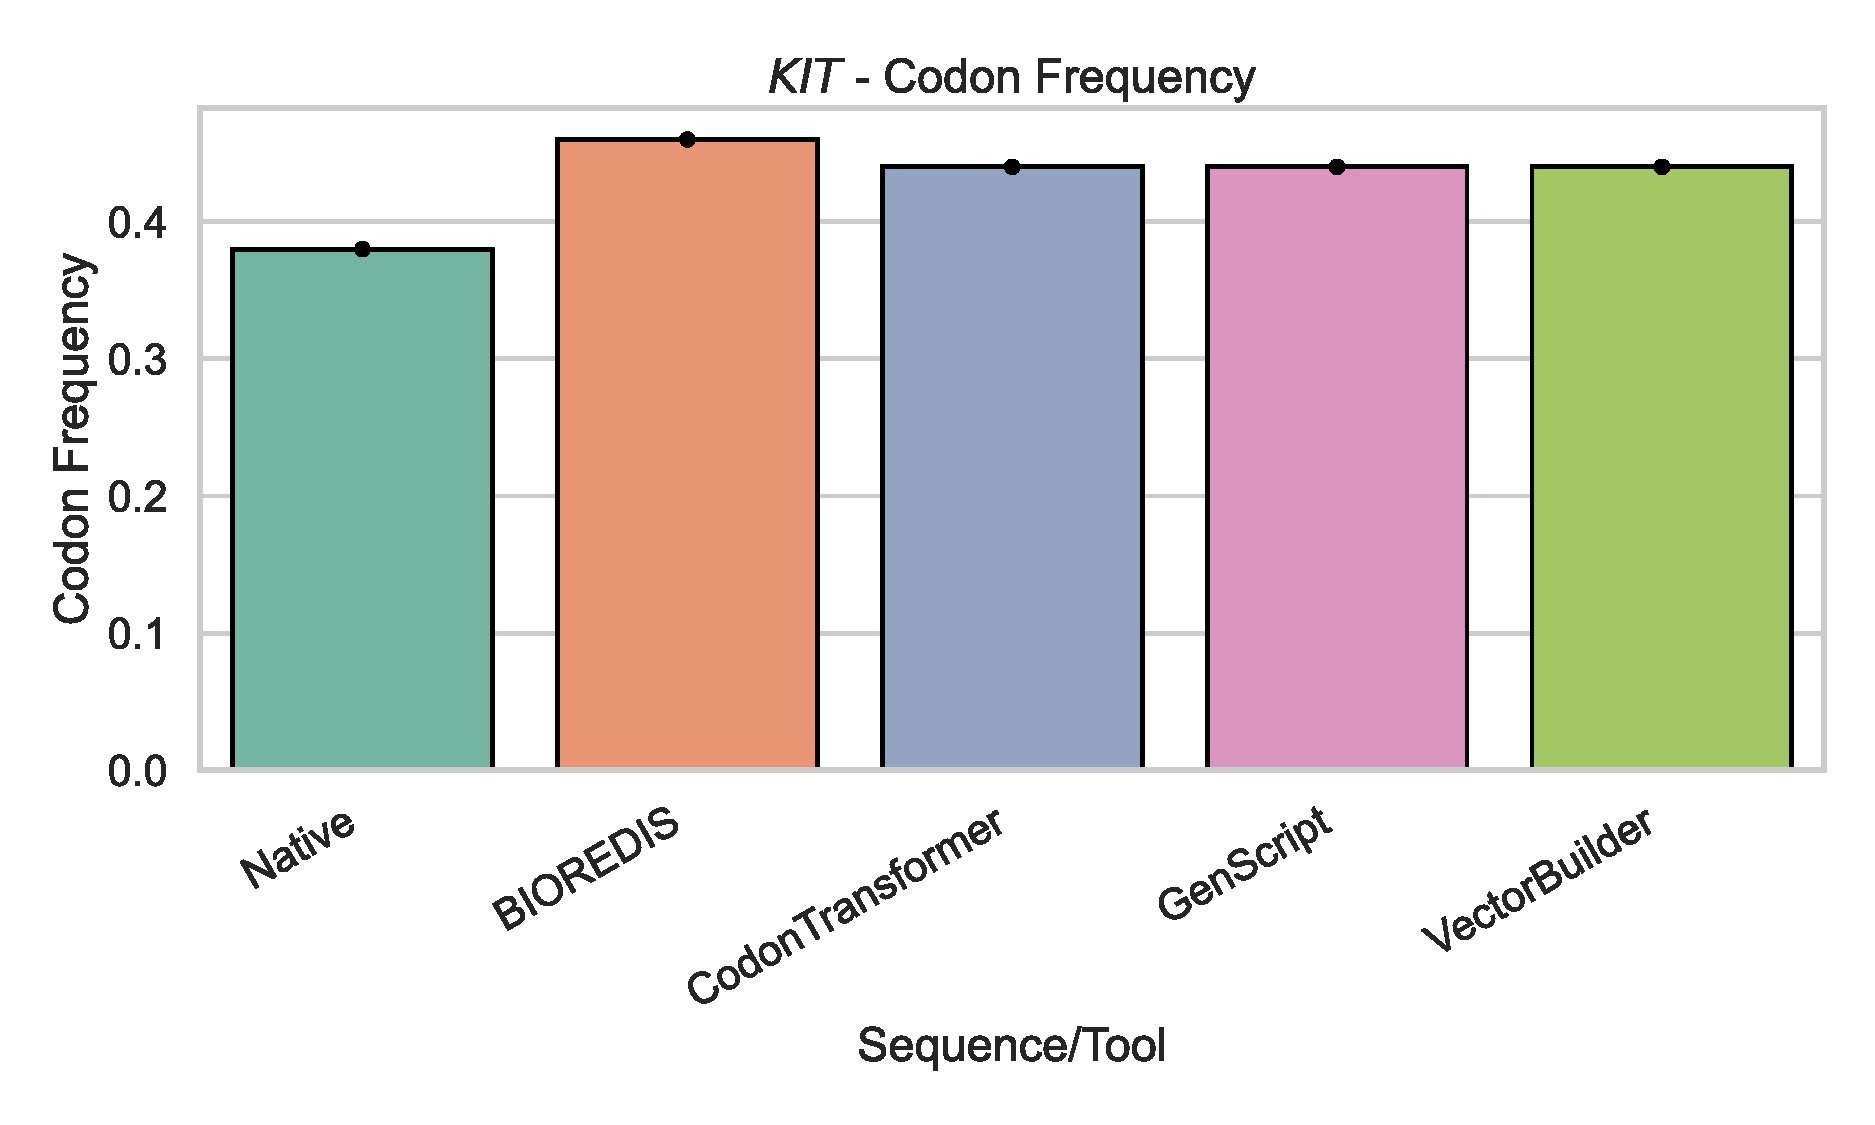
\includegraphics[width=0.8\linewidth]{supplemetary_figures/Supp.Fig.3-KIT} \end{center}

\begin{center}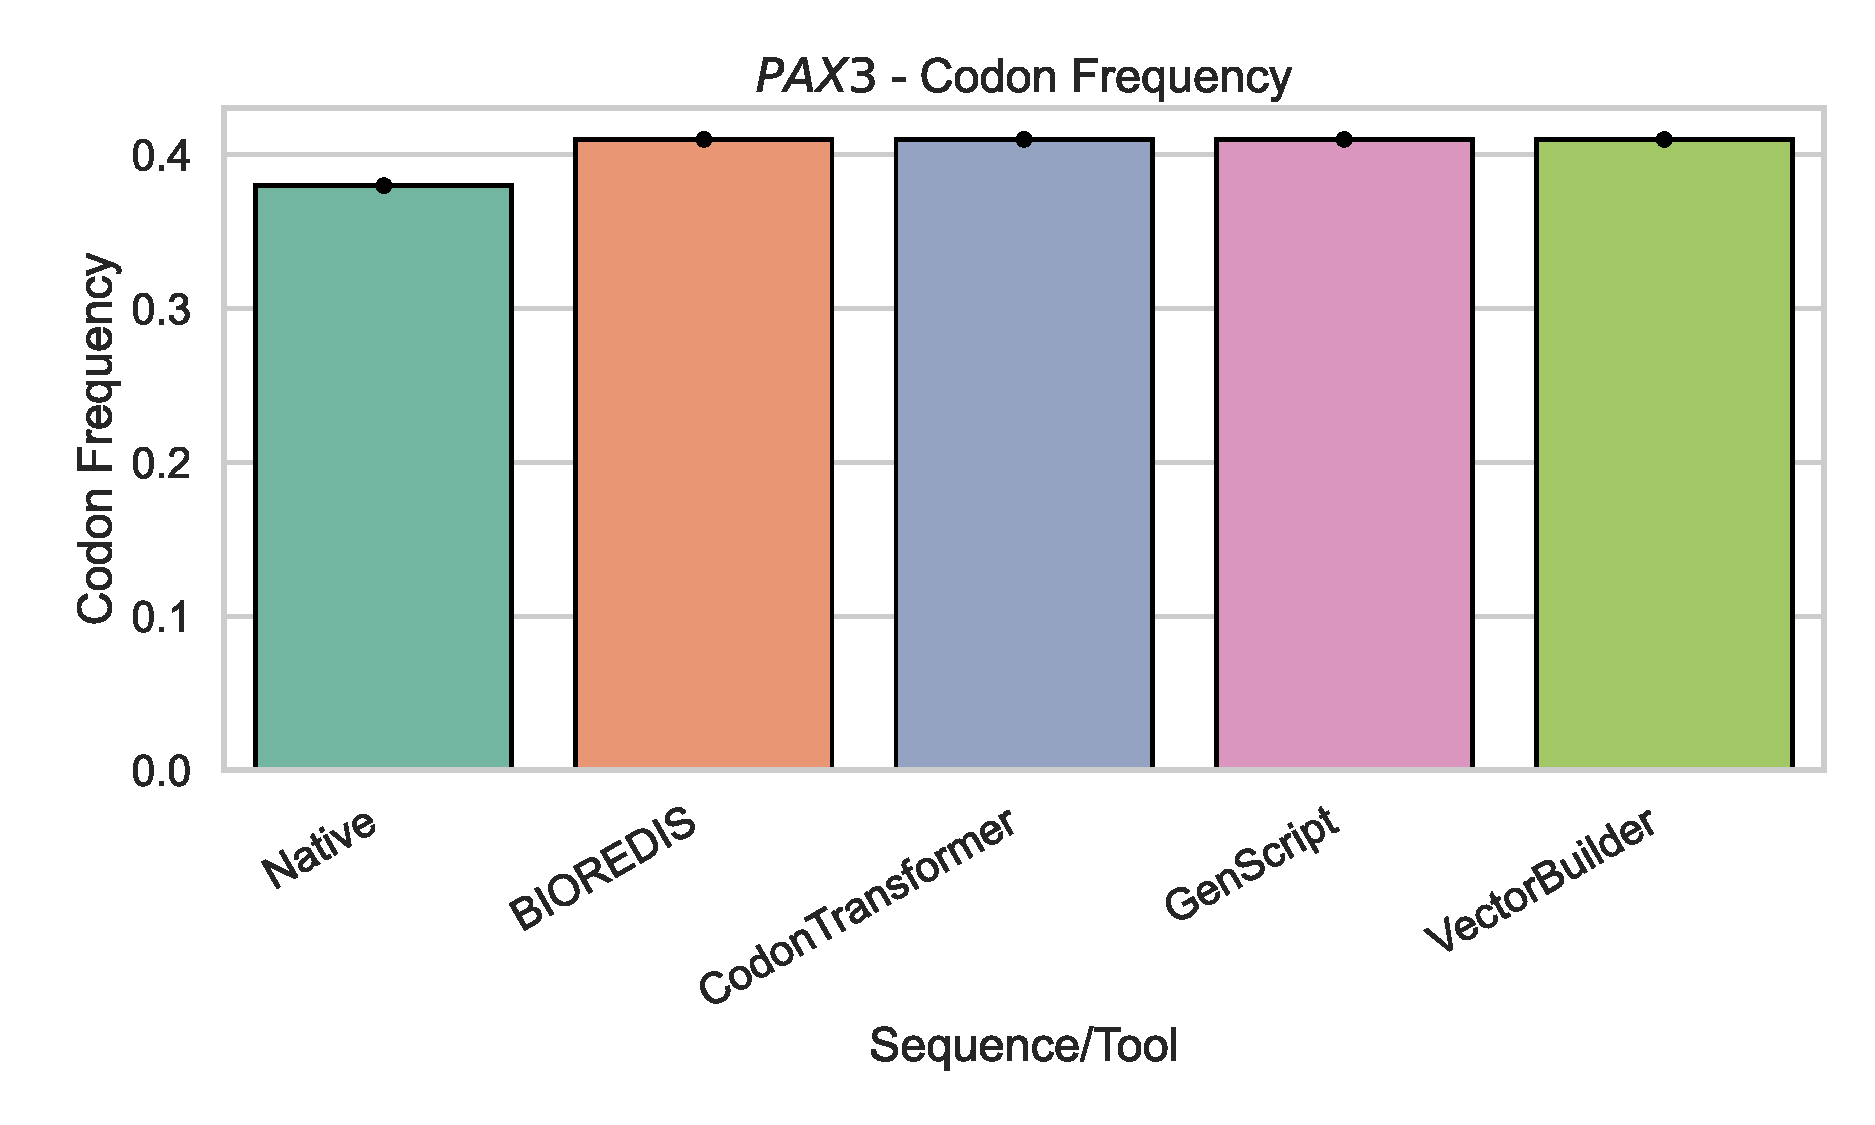
\includegraphics[width=0.8\linewidth]{supplemetary_figures/Supp.Fig.3-PAX3} \end{center}

\textbf{Figure S3.} Codon frequency values in optimised and native
sequences of the \emph{KIT} and \emph{PAX3} genes

\newpage

\begin{center}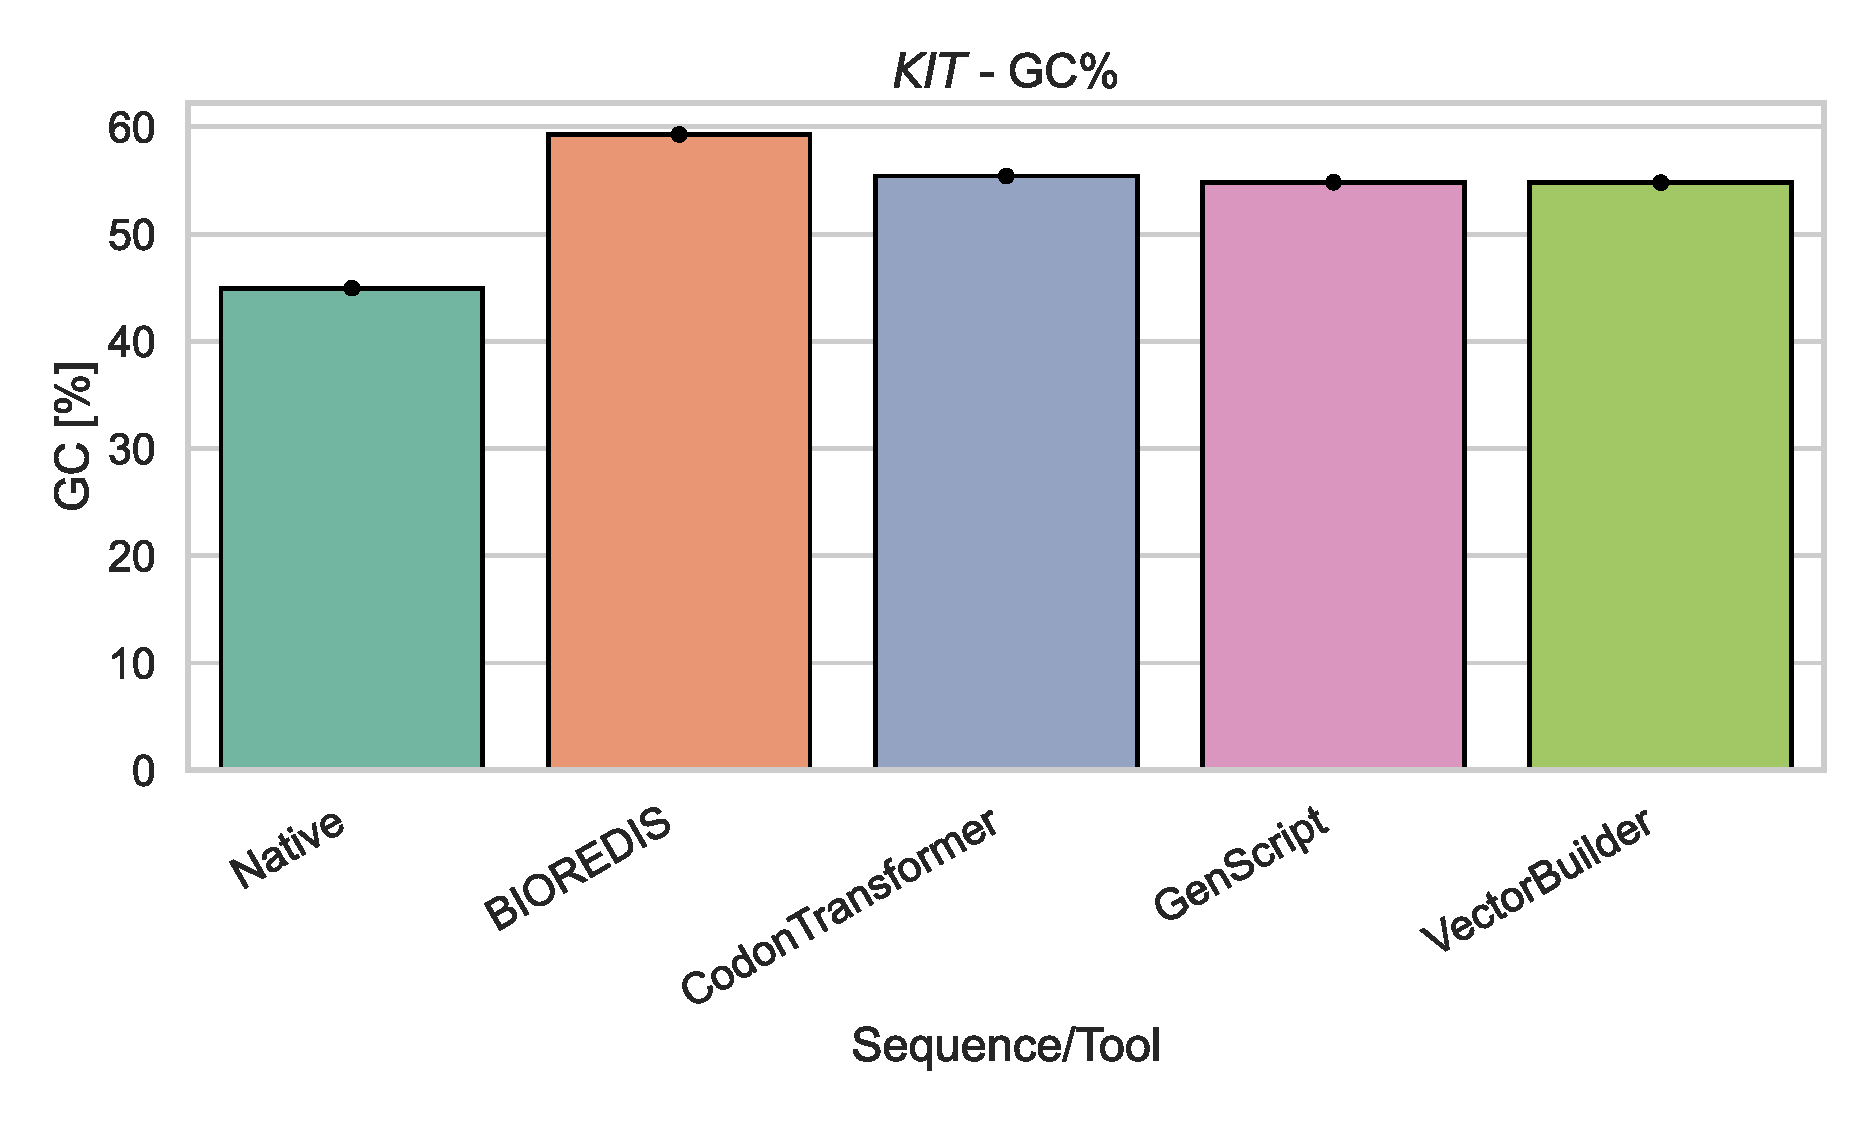
\includegraphics[width=0.8\linewidth]{supplemetary_figures/Supp.Fig.4-KIT} \end{center}

\begin{center}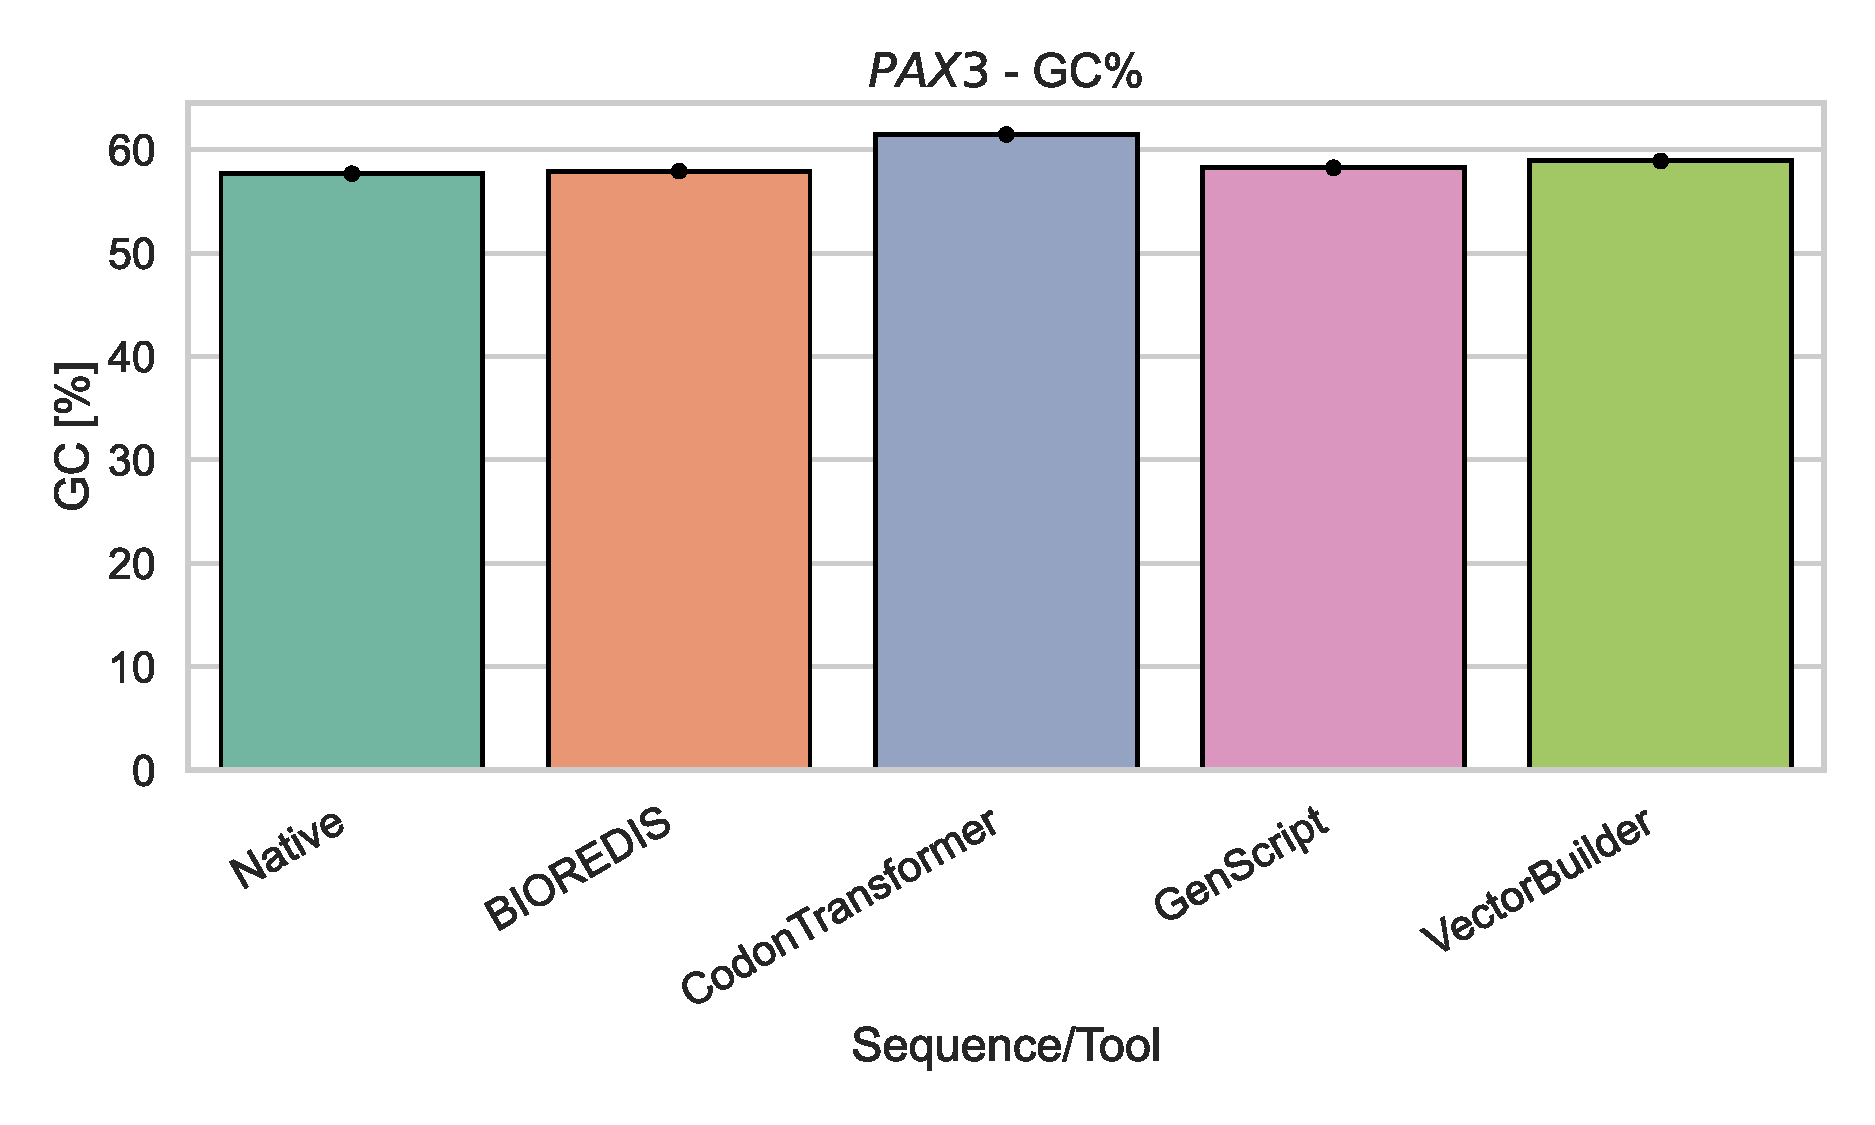
\includegraphics[width=0.8\linewidth]{supplemetary_figures/Supp.Fig.4-PAX3} \end{center}

\textbf{Figure S4.} GC content {[}\%{]} in optimised and native
sequences of the \emph{KIT} and \emph{PAX3} genes

\newpage

\begin{center}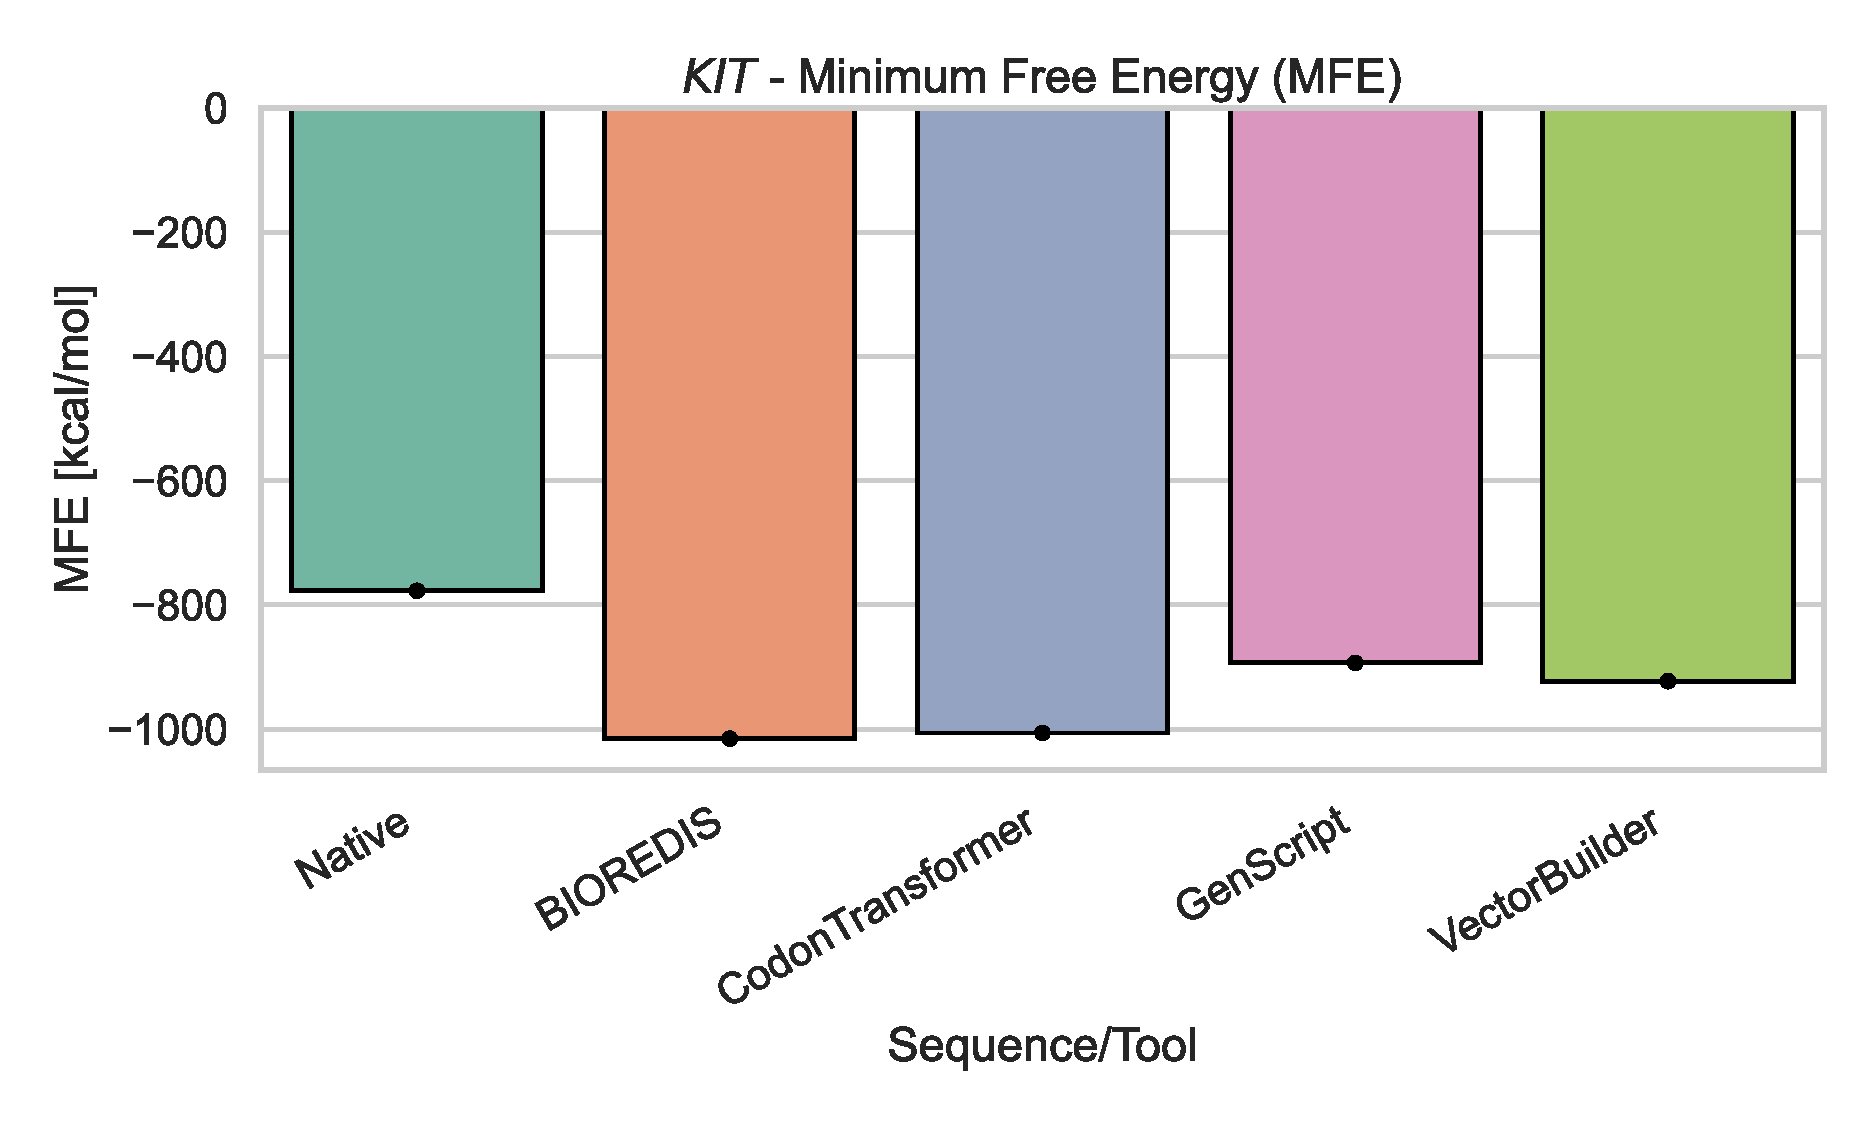
\includegraphics[width=0.8\linewidth]{supplemetary_figures/Supp.Fig.5-KIT} \end{center}

\begin{center}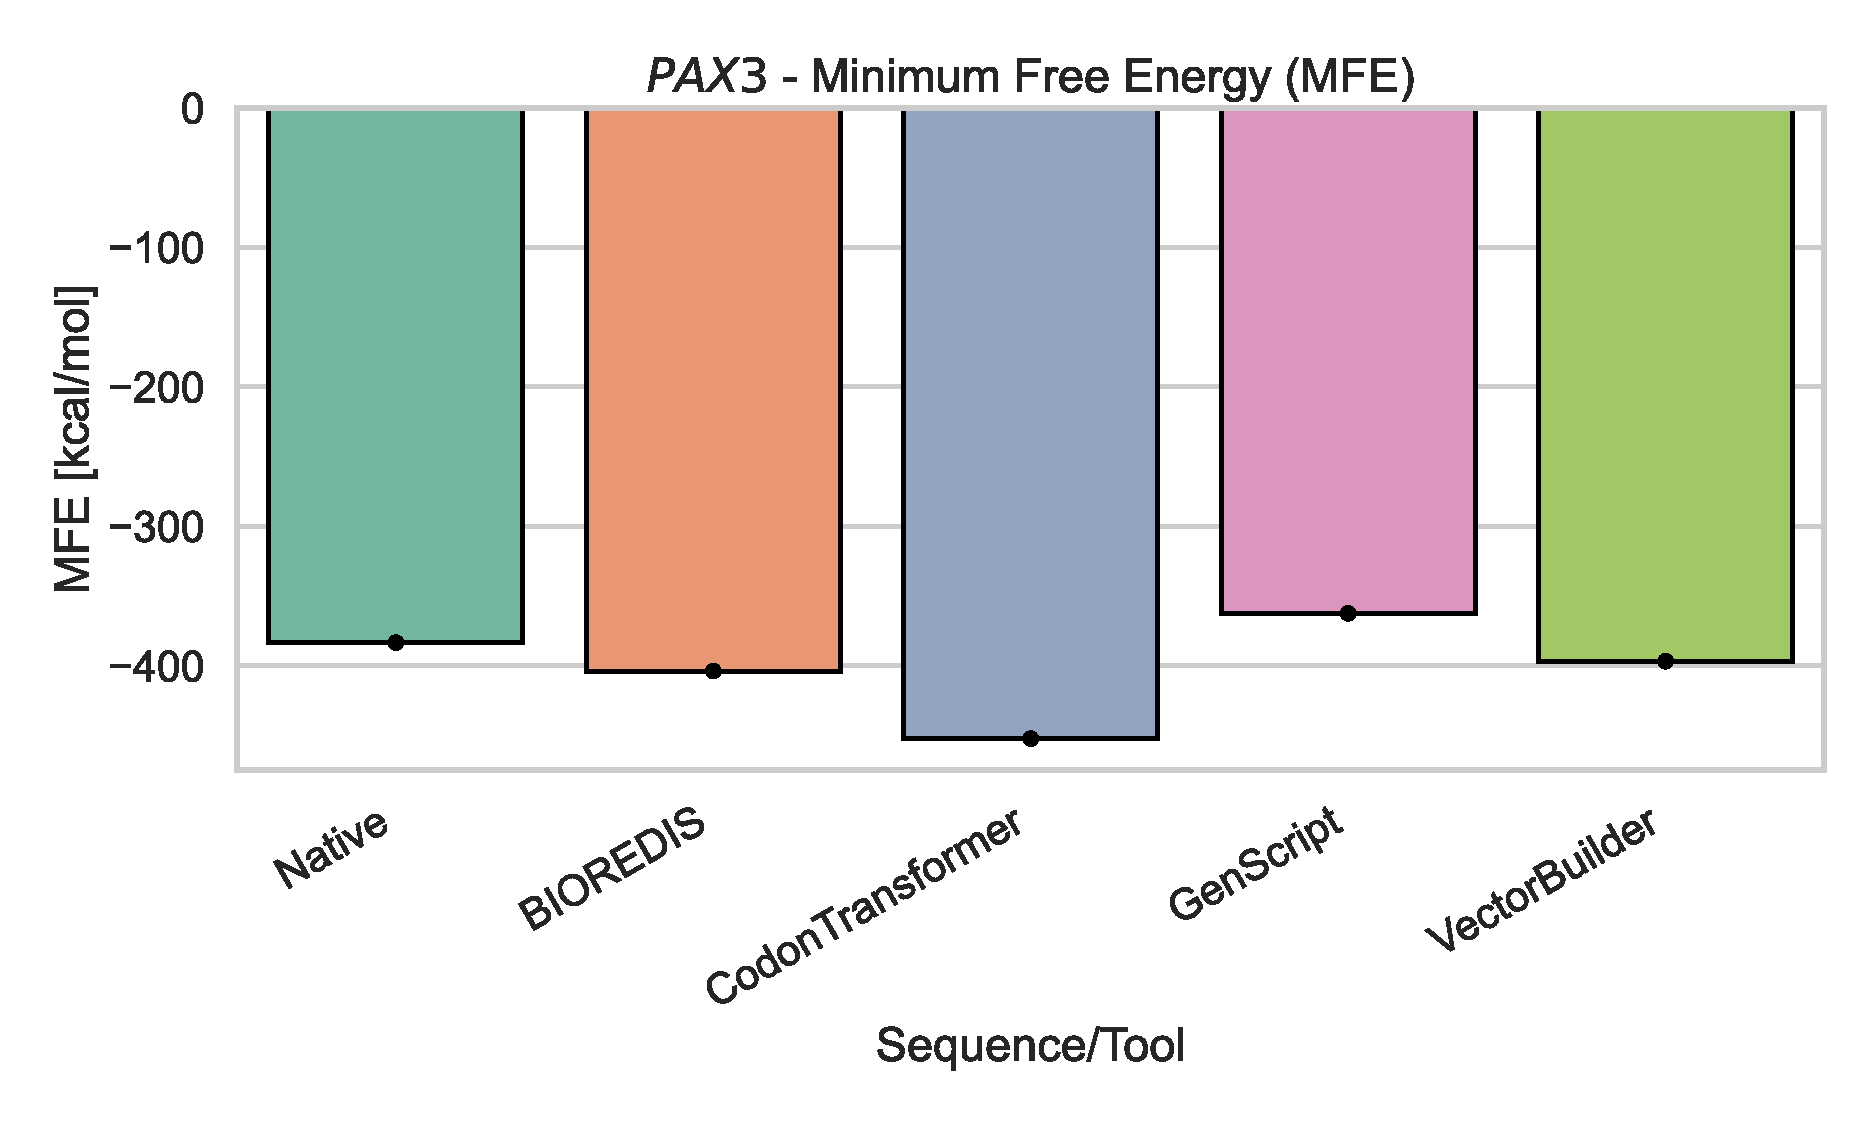
\includegraphics[width=0.8\linewidth]{supplemetary_figures/Supp.Fig.5-PAX3} \end{center}

\textbf{Figure S5.} MFE {[}Minimum Free Energy{]} values in optimised
and native sequences of the \emph{KIT} and \emph{PAX3} genes

\newpage

\begin{center}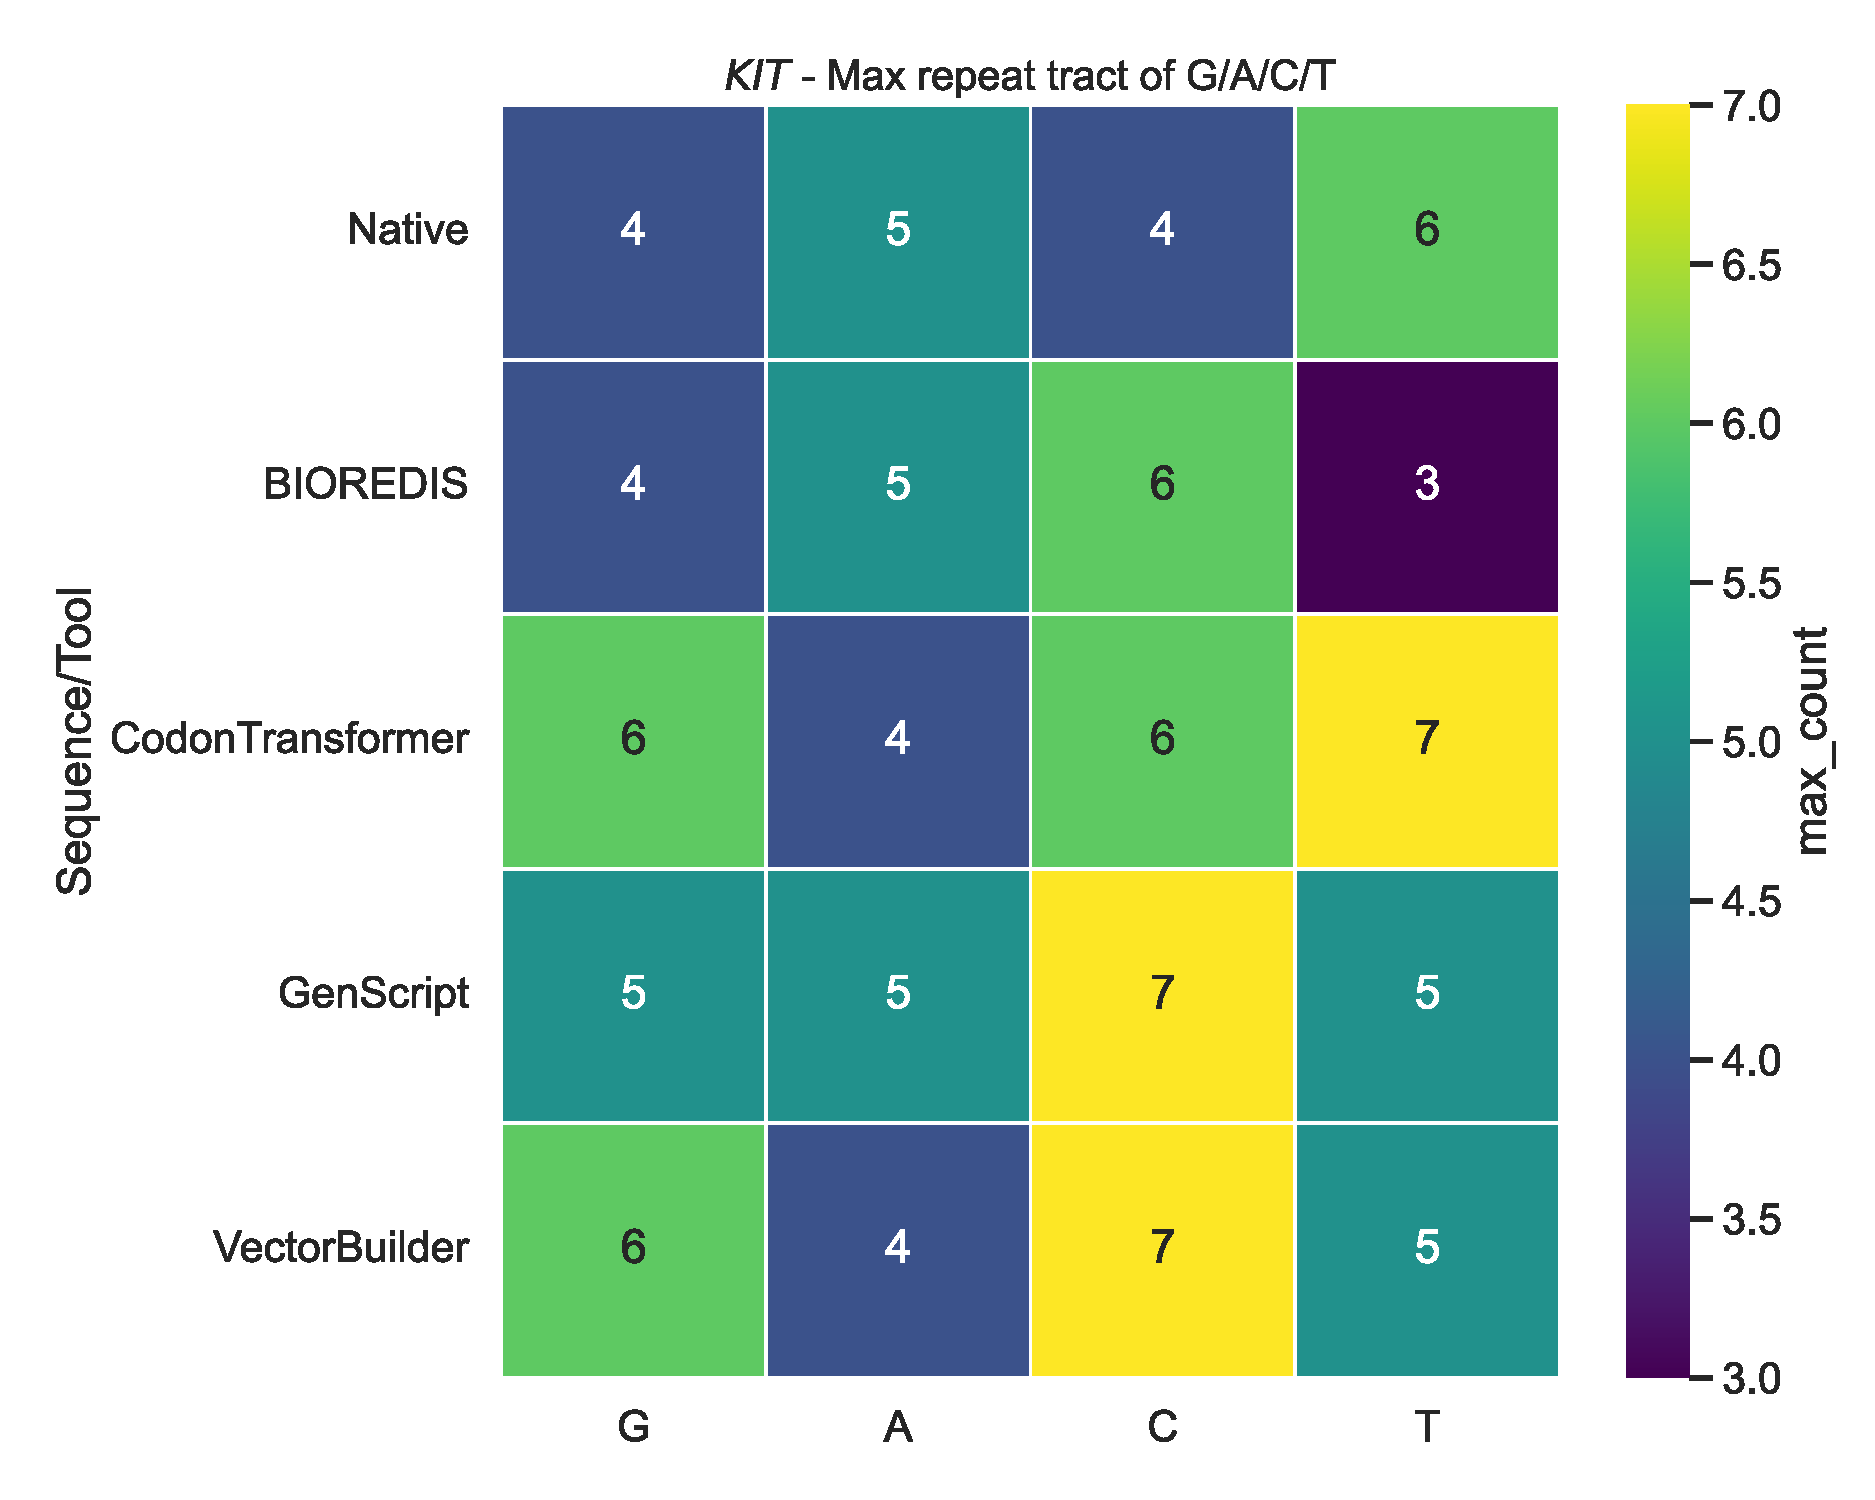
\includegraphics[width=0.8\linewidth]{supplemetary_figures/Supp.Fig.6-KIT} \end{center}

\begin{center}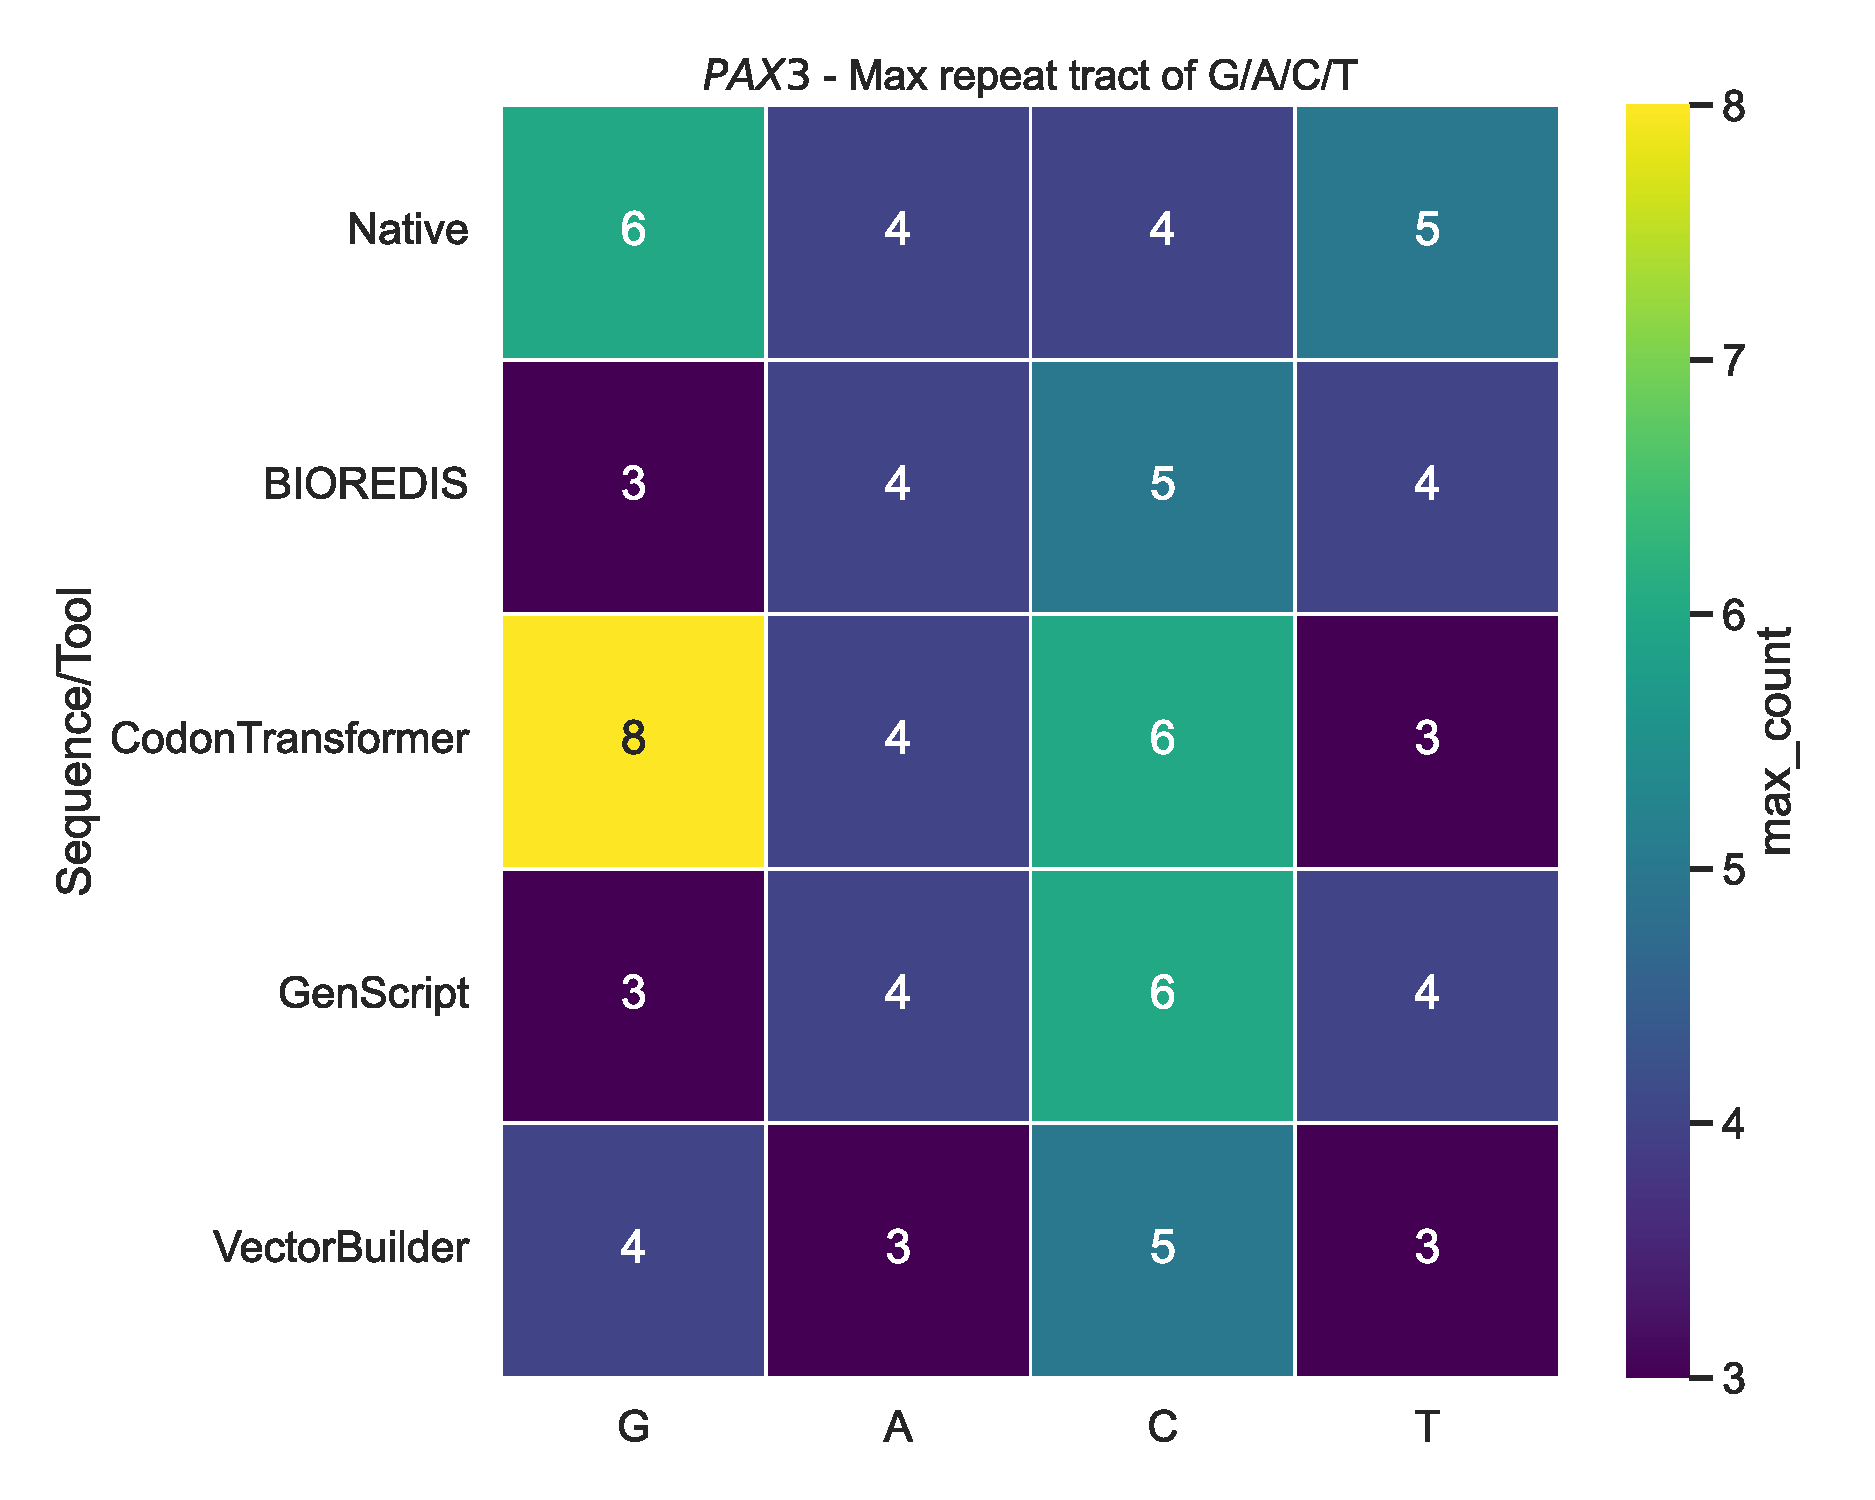
\includegraphics[width=0.8\linewidth]{supplemetary_figures/Supp.Fig.6-PAX3} \end{center}

\textbf{Figure S6.} Heatmap of longest consecutive A/C/T/G tracts in
optimised sequences of the \emph{KIT} and \emph{PAX3} genes.

\newpage

\subsection{RNAi (siRNA/shRNA)
prediction}\label{rnai-sirnashrna-prediction}

\begin{center}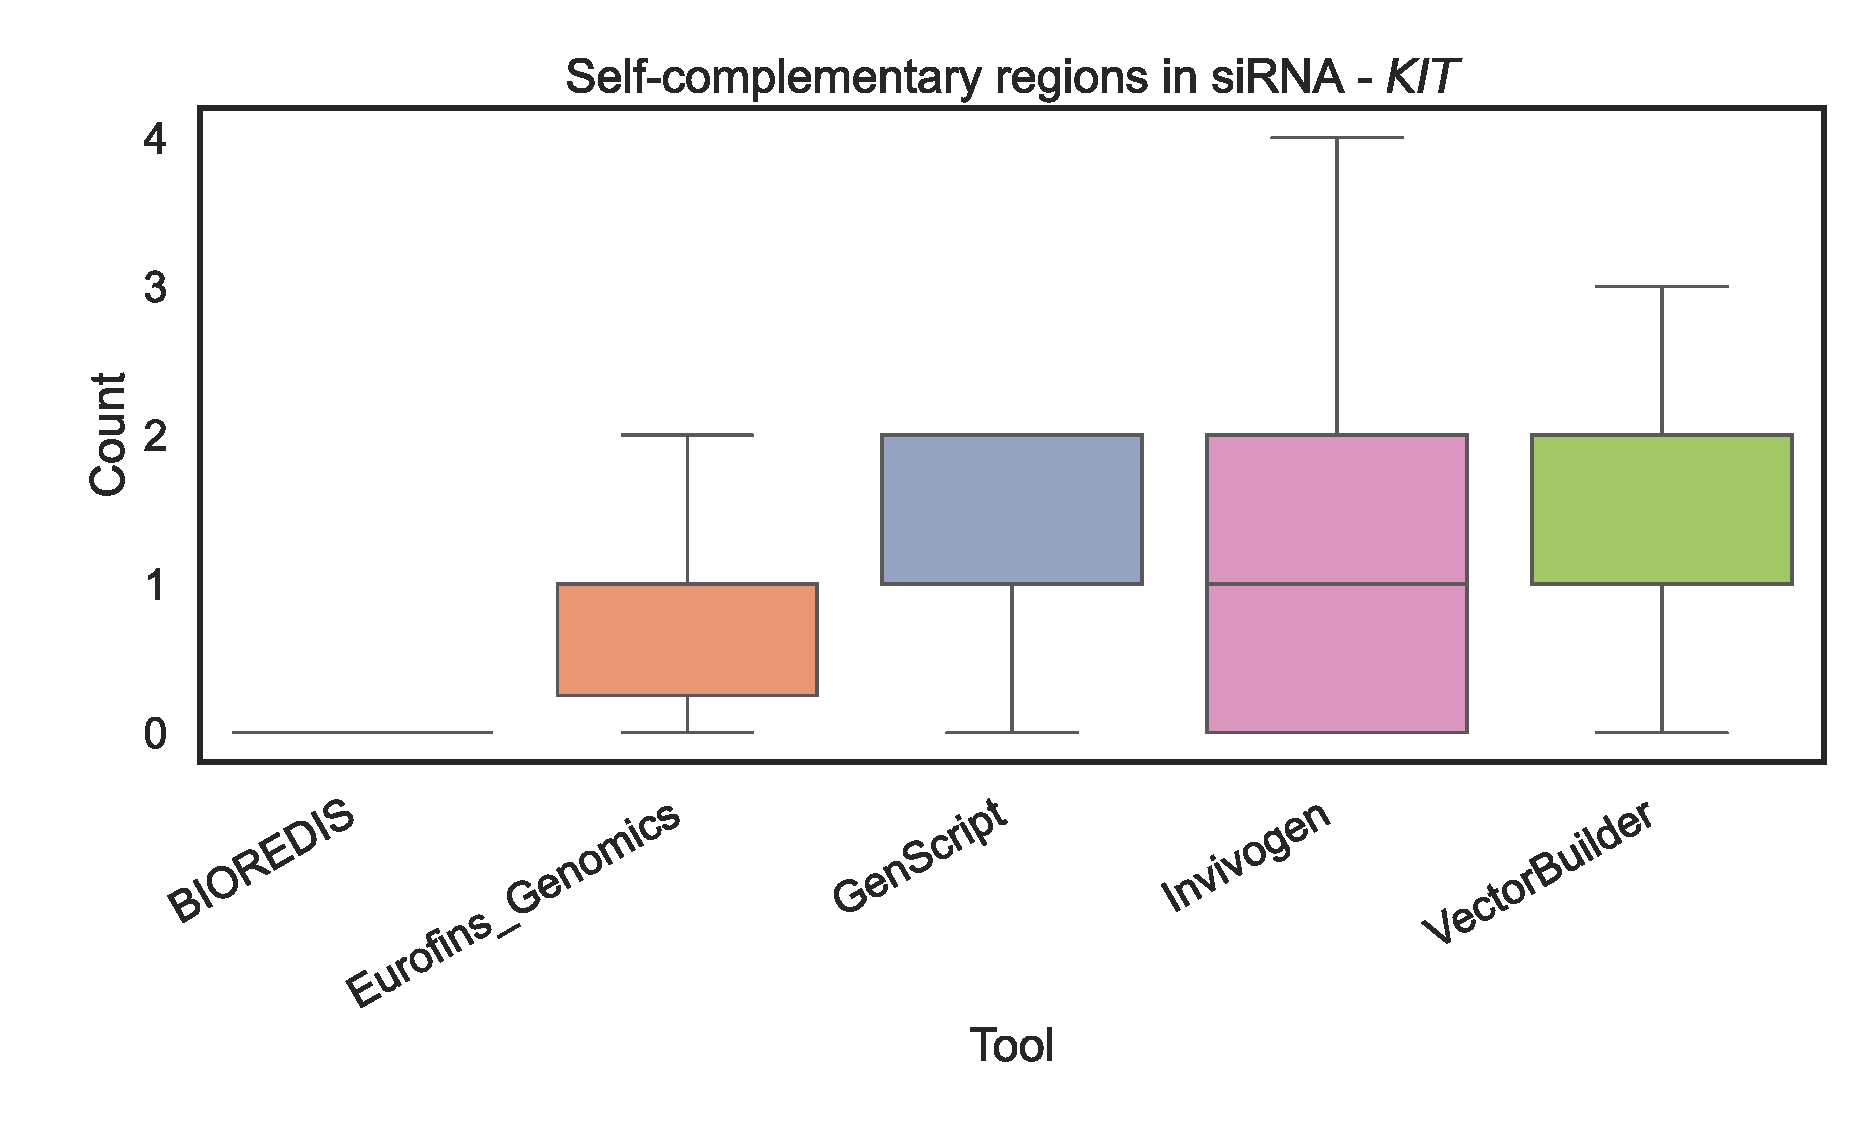
\includegraphics[width=0.8\linewidth]{supplemetary_figures/Supp.Fig.7-KIT} \end{center}

\begin{center}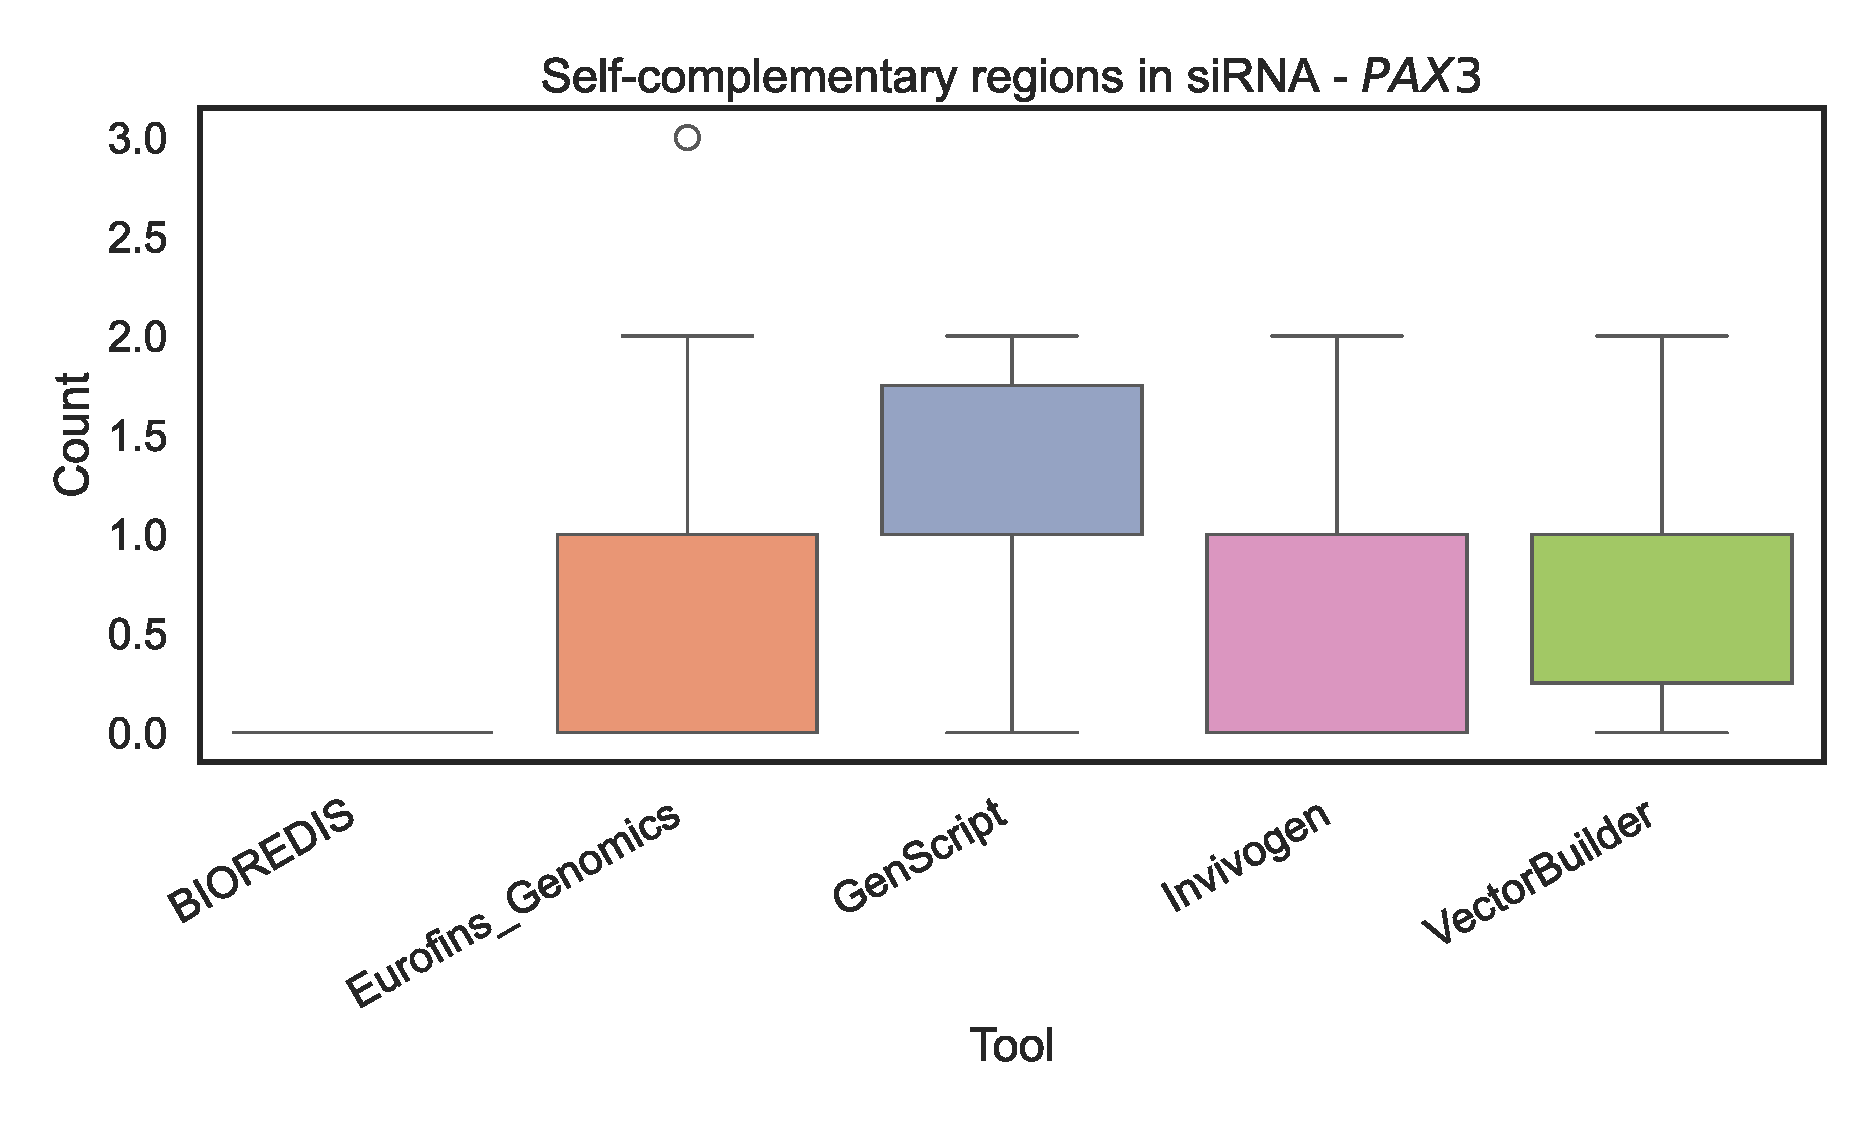
\includegraphics[width=0.8\linewidth]{supplemetary_figures/Supp.Fig.7-PAX3} \end{center}

\textbf{Figure S7.} Counts of self-complementary regions in predicted
RNAi sequences targeting the \emph{KIT} and \emph{PAX3} genes.

\newpage

\begin{center}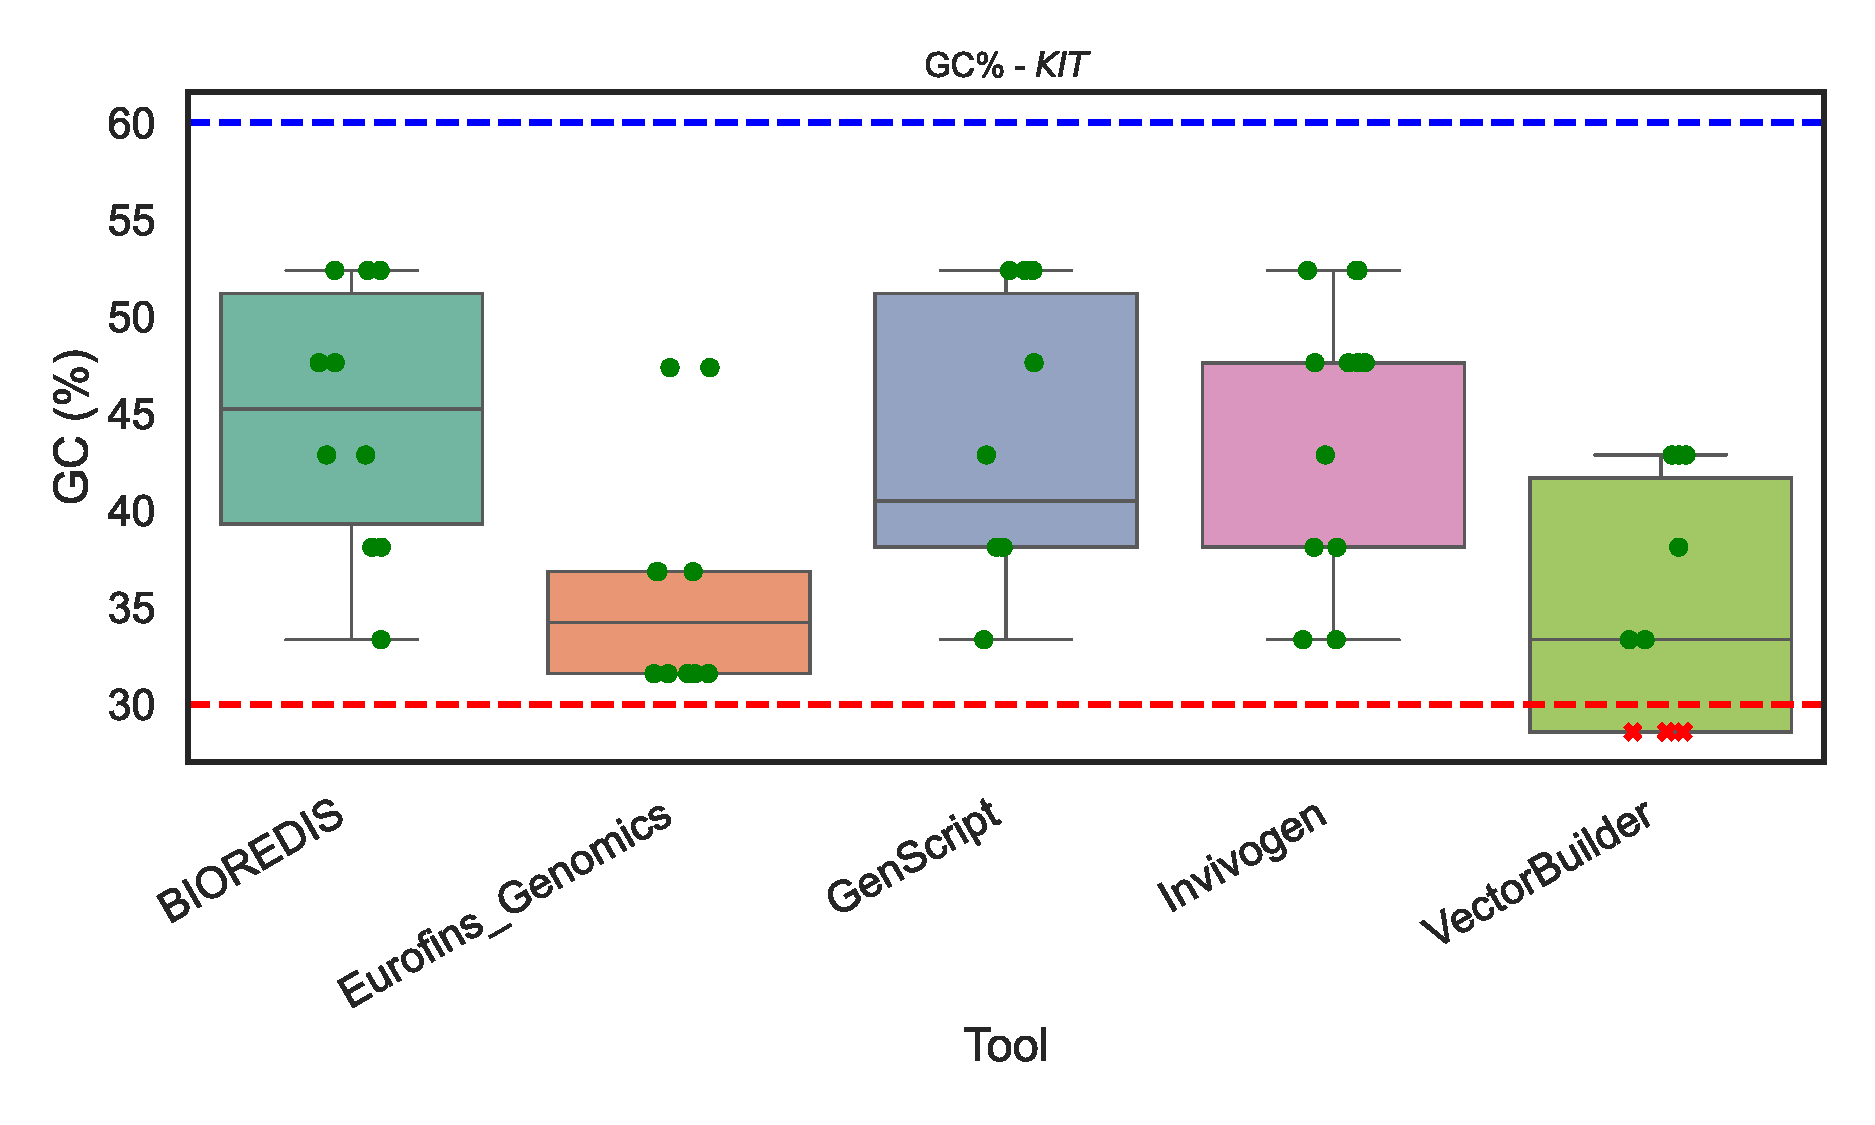
\includegraphics[width=0.8\linewidth]{supplemetary_figures/Supp.Fig.8-KIT} \end{center}

\begin{center}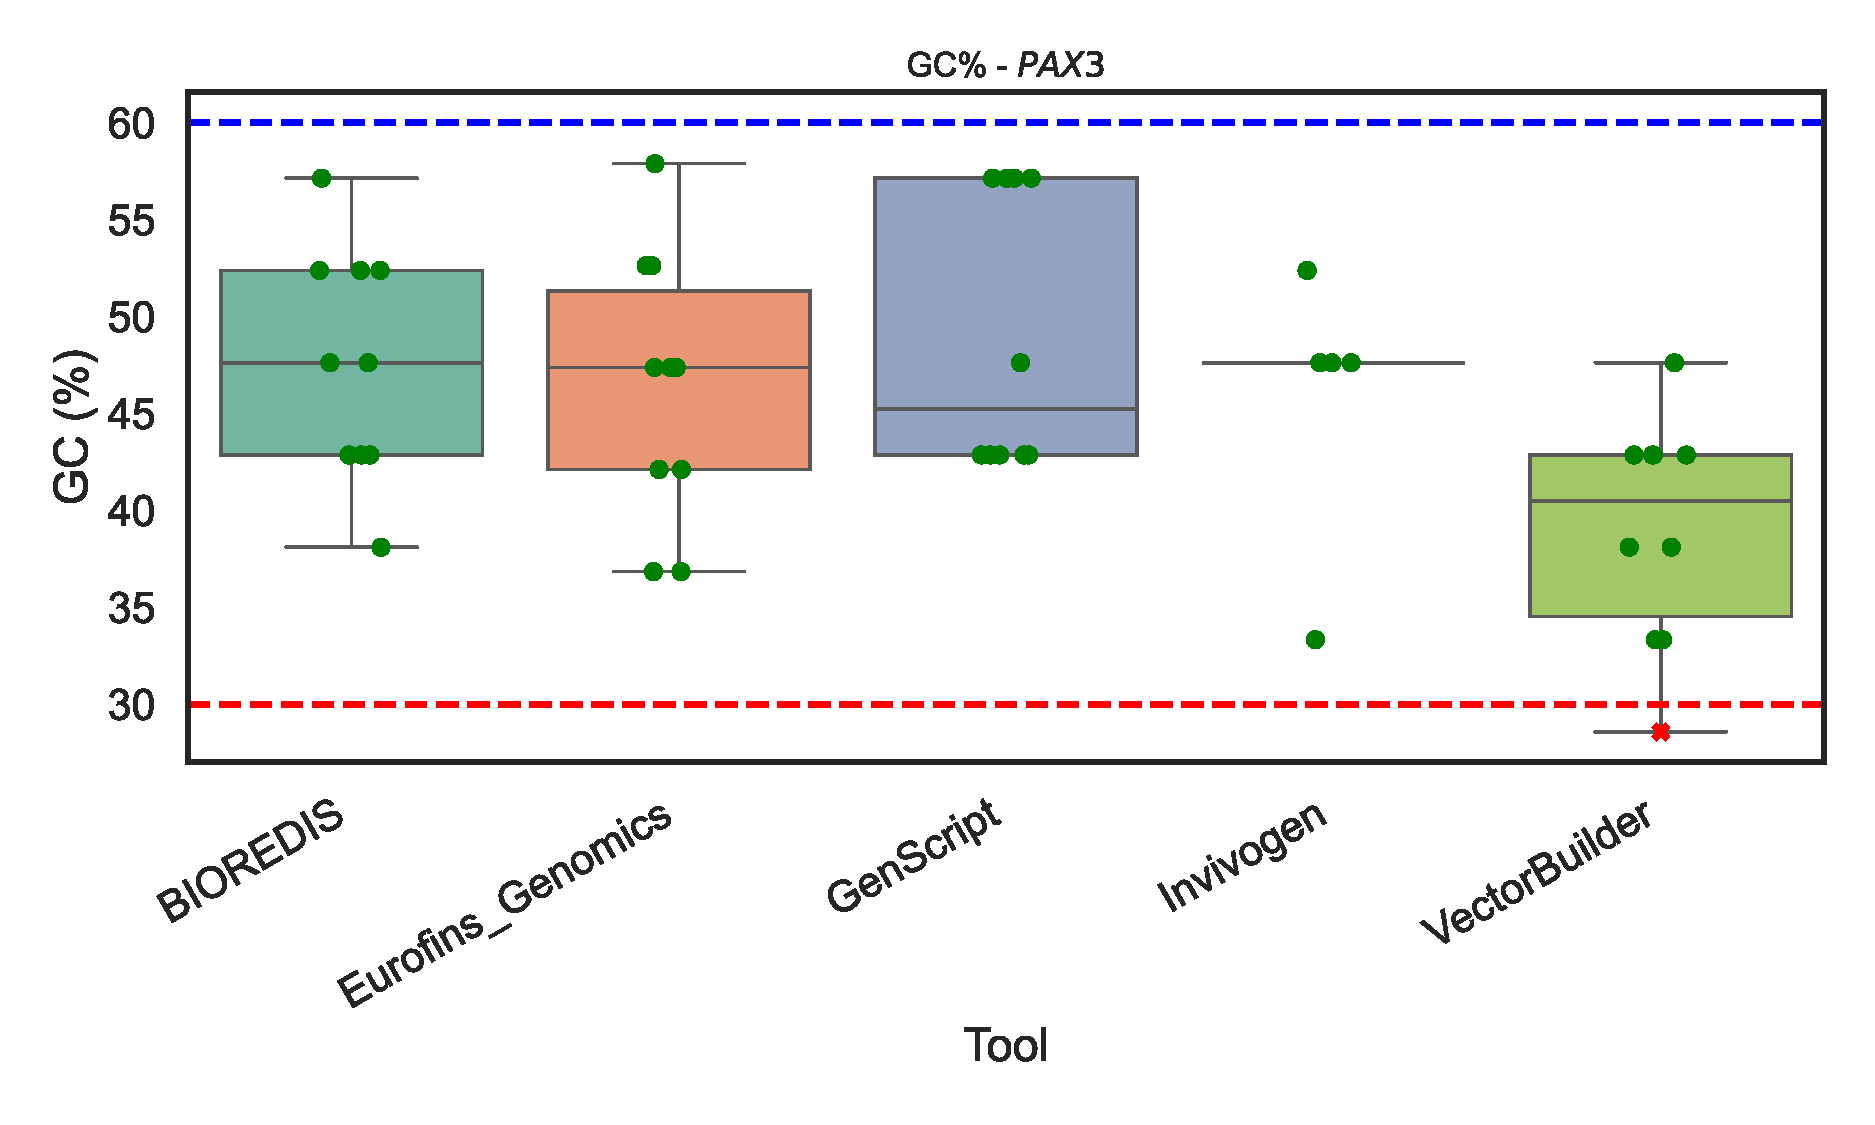
\includegraphics[width=0.8\linewidth]{supplemetary_figures/Supp.Fig.8-PAX3} \end{center}

\textbf{Figure S8.} GC content {[}\%{]} in predicted RNAi sequences
targeting the \emph{KIT} and \emph{PAX3} genes.

\newpage

\begin{center}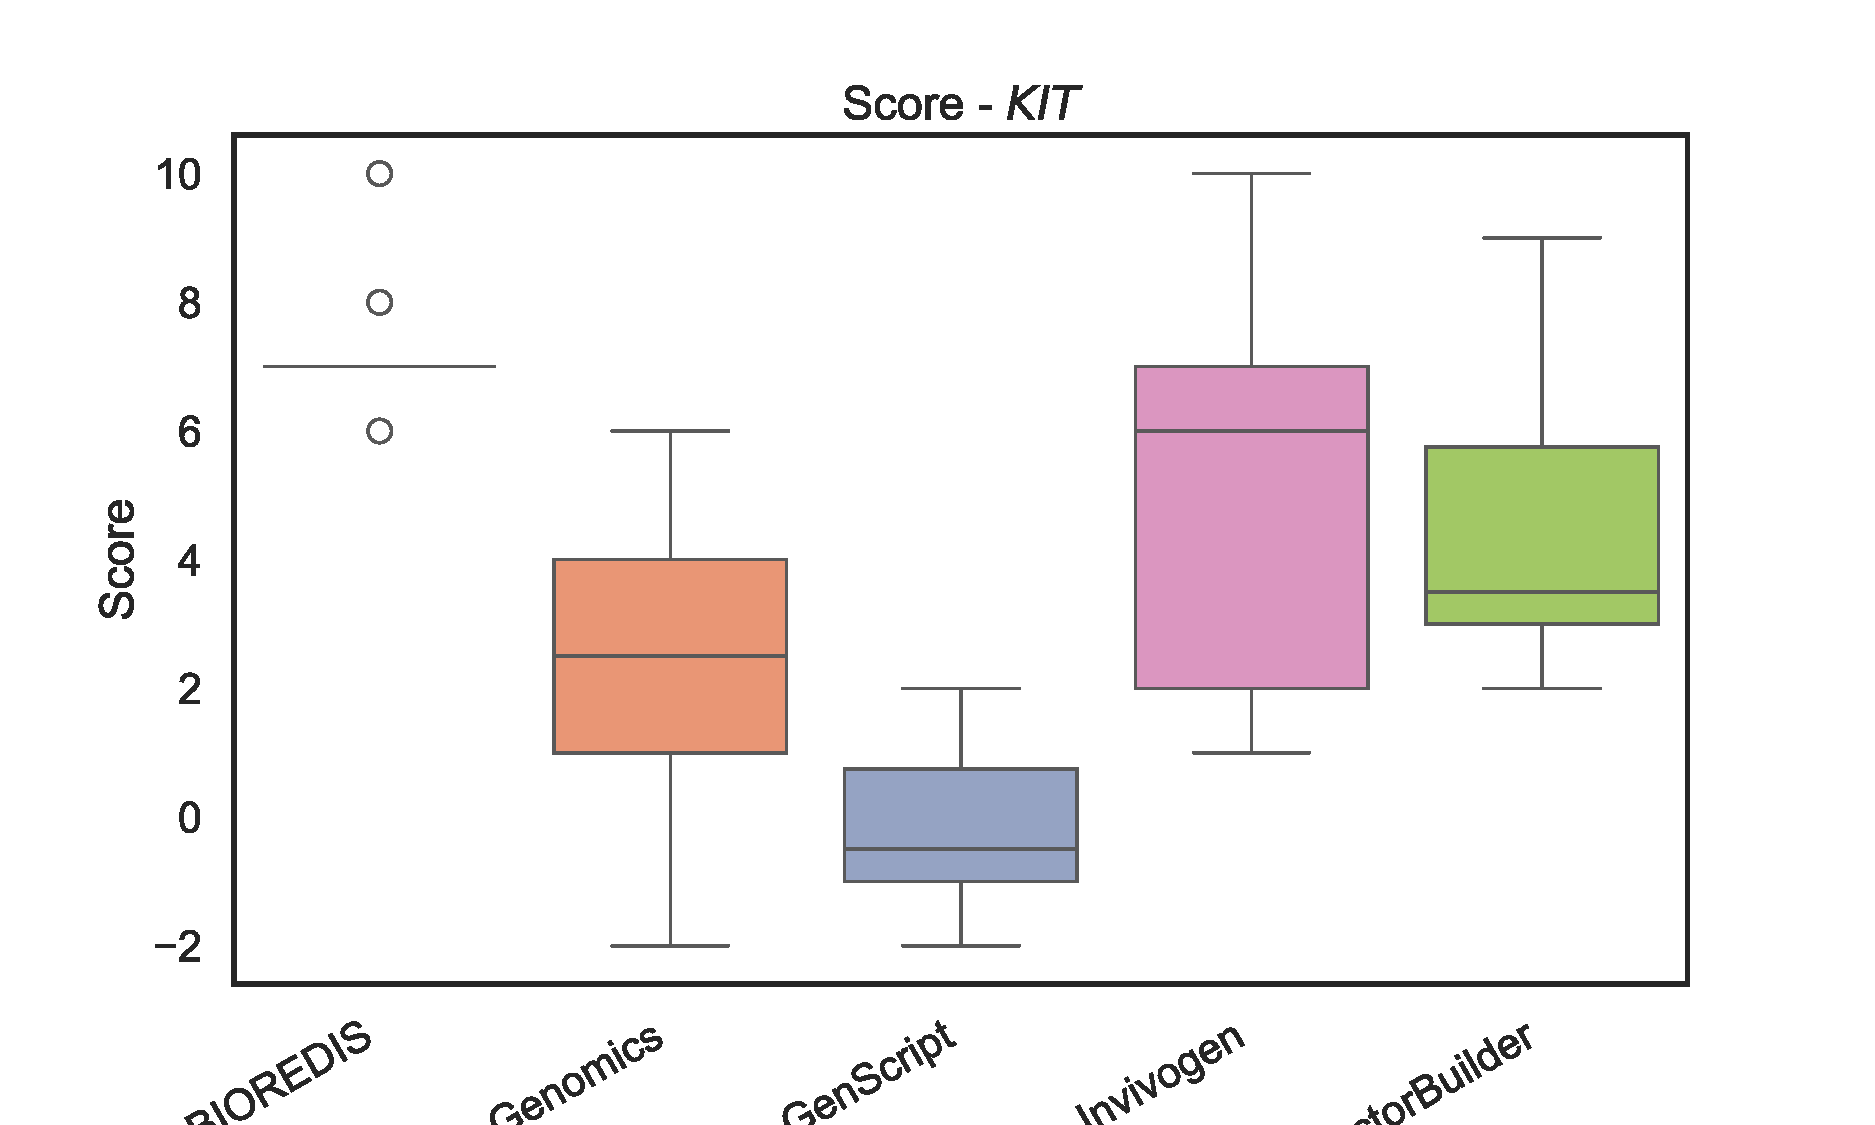
\includegraphics[width=0.8\linewidth]{supplemetary_figures/Supp.Fig.9-KIT} \end{center}

\begin{center}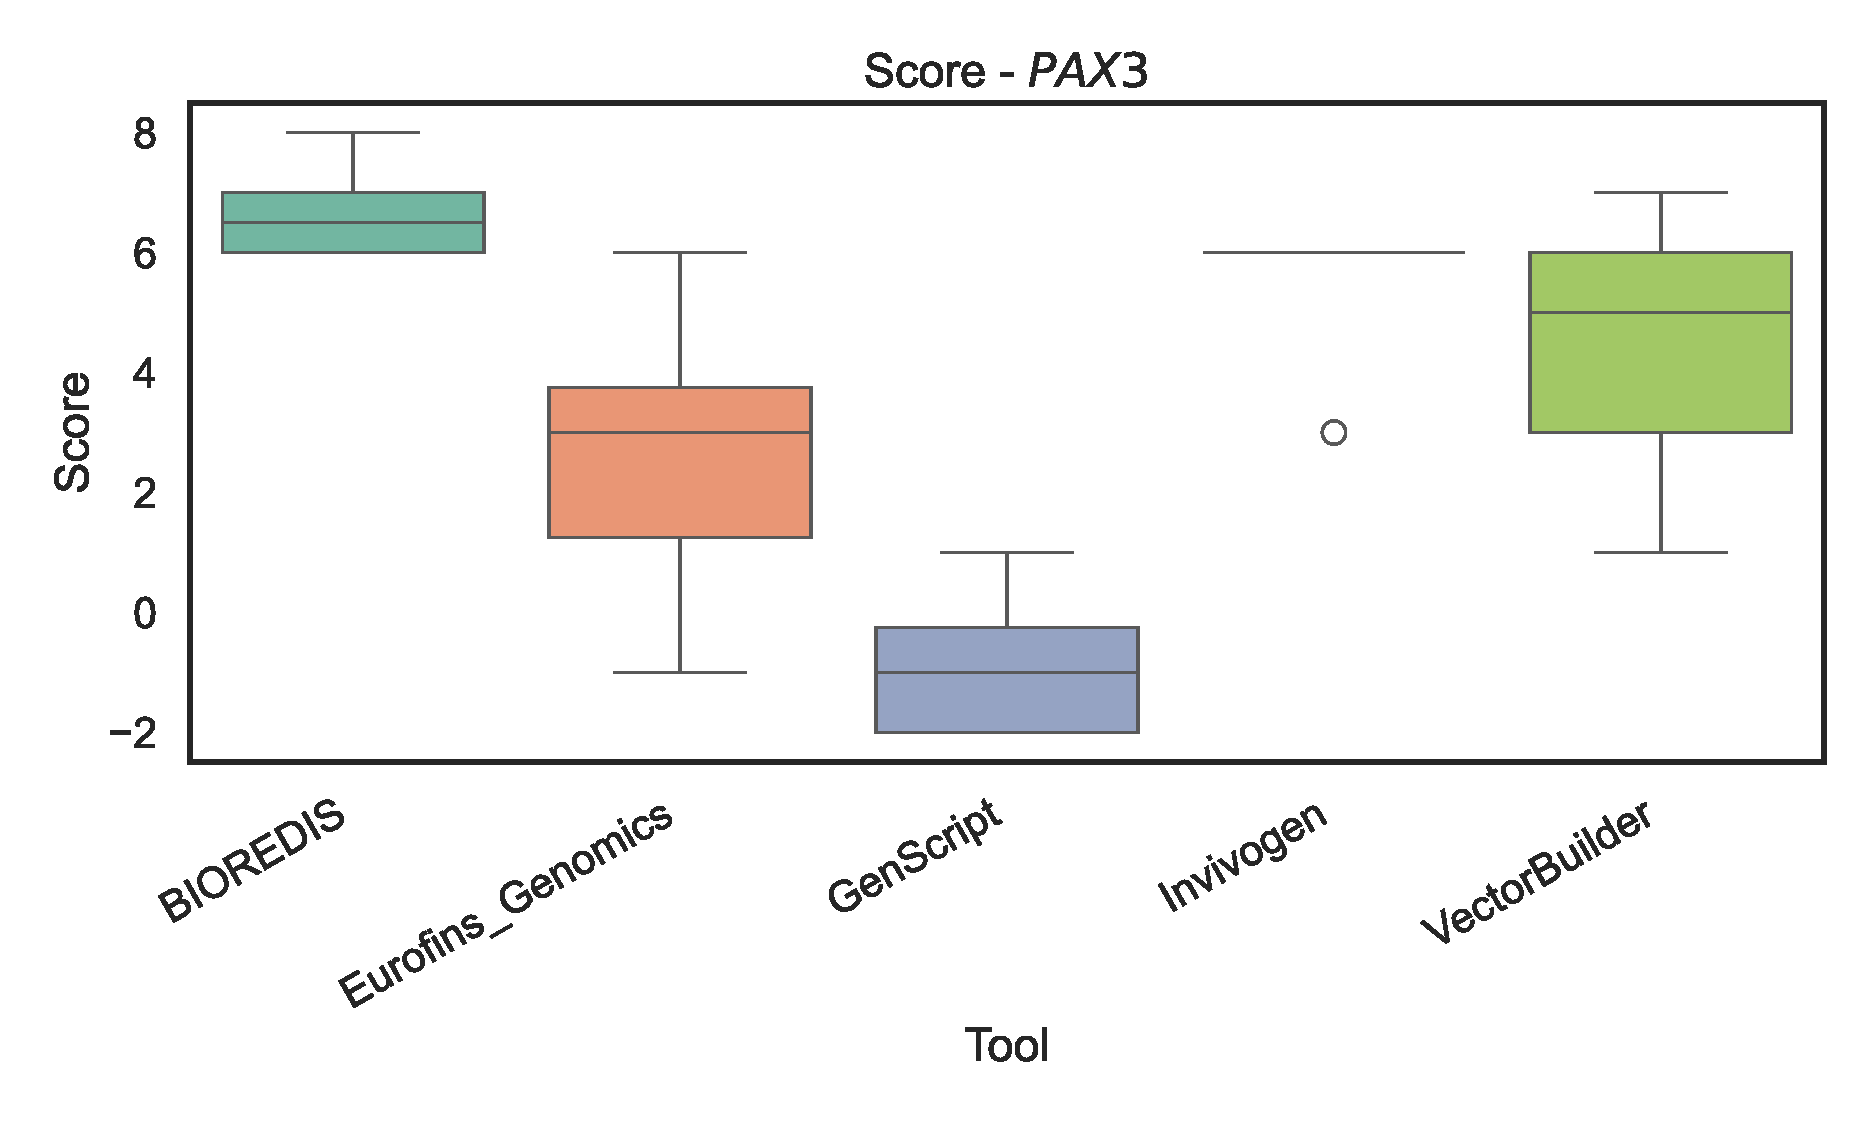
\includegraphics[width=0.8\linewidth]{supplemetary_figures/Supp.Fig.9-PAX3} \end{center}

\textbf{Figure S9.} Nucleotide positions score in predicted RNAi
sequences targeting the \emph{KIT} and \emph{PAX3} genes based on series
of publications: \url{DOI:10.1093/nar/gkn902};
\url{DOI:10.1093/nar/gkh247}; \url{DOI:10.1038/nbt936};;
\url{DOI:10.1016/j.bbrc.2004.02.157}

\end{document}
